\documentclass[11pt,twoside,openright]{book}

\usepackage[
  paperwidth=17cm,
  paperheight=24cm,
  top=3cm,
  bottom=2.5cm,
  left=2.5cm,
  right=2cm,
  twoside
]{geometry}

\usepackage[T1]{fontenc}
\usepackage{lmodern}
\usepackage[english]{babel}
\usepackage{graphicx}
\usepackage{pdfpages}
\usepackage{xcolor}
\usepackage{microtype}
\usepackage{amsmath,amssymb,amsfonts}
\usepackage{booktabs}
\usepackage{array}
\usepackage{caption}
\usepackage{csquotes}
\usepackage{titlesec}
\usepackage{fancyhdr}
\usepackage[hidelinks,bookmarksnumbered]{hyperref}
\usepackage{bookmark}
\usepackage{tcolorbox}
\usepackage{enumitem}
\usepackage[
  backend=biber,
  dashed=false,
  style=ieee,
  defernumbers=true,
  sorting=none,
  maxbibnames=99,
  url=false
]{biblatex}

\addbibresource{references/thesis.bib}
\addbibresource{references/my_contribution.bib}

\setlength{\parskip}{0pt plus 4pt}
\setlength{\headheight}{14pt}

\renewcommand{\thechapter}{\arabic{chapter}}
\titleformat{\chapter}[display]
  {\Large}
  {\filleft\MakeUppercase{\chaptertitlename}\ \Huge\thechapter}
  {2ex}
  {\titlerule\vspace{2ex}\bfseries\filleft\huge}
  [\vspace{1.3ex}\titlerule]

% Keep running heads short so a long chapter/section title can never collide
% with the page number on the opposite side of the header.
\renewcommand{\chaptermark}[1]{\markboth{\chaptername\ \thechapter.\ #1}{}}
\renewcommand{\sectionmark}[1]{\markright{\thesection\ #1}}

\fancyhf{}
\fancyhead[LE,RO]{\small\thepage}
\fancyhead[RE]{\small\nouppercase{\leftmark}}
\fancyhead[LO]{\small\nouppercase{\rightmark}}
\fancyfoot{}
\renewcommand{\headrulewidth}{0.5pt}
\renewcommand{\footrulewidth}{0pt}

\captionsetup{font=small}

% --- Publication cover page ----------------------------------------------------
% Prints a dedicated page that announces the next included paper by its title and
% full bibliographic reference, immediately before the paper PDF is embedded.
% Usage: \publicationcover{<my_contribution bib key>}
\newcommand{\publicationcover}[1]{%
  \cleardoublepage
  \thispagestyle{empty}%
  {\centering
    \vspace*{0.22\textheight}
    {\large\scshape Included Publication\par}
    \vspace{3ex}
    {\Large\bfseries \citetitle*{#1}\par}
    \vspace{3ex}
    \rule{0.6\textwidth}{0.4pt}\par
  }
  \vfill
  {\small
    \noindent\textbf{Full reference:}\par
    \vspace{0.5ex}
    \noindent\fullcite{#1}\par
  }
  \vspace{0.12\textheight}
  \clearpage
}


\newcommand{\ThesisTitle}{Cross-Layer Network Security\\ in the Post-Quantum Era}
\newcommand{\ThesisSubtitle}{From Integrated Quantum Sources\\ to Datacenter-Scale Cryptography}
\newcommand{\ThesisAuthor}{Joseph Gideon Meyer}
\newcommand{\ThesisDefenseDate}{dinsdag 6 oktober 2026 om 16:00 uur}
\newcommand{\ThesisBirthLine}{geboren te Toronto, Ontario, Canada}

\begin{document}

\frontmatter
\pagestyle{empty}

\thispagestyle{empty}
{\large
\begin{center}
    \null\vfill

    {\LARGE\ThesisTitle\par}

    \vspace{0.6em}

    {\large\itshape\ThesisSubtitle\par}

    \vfill

    PROEFSCHRIFT

    \vfill

    \begin{minipage}{0.82\textwidth}
      \righthyphenmin=1000000
      \lefthyphenmin=1000000
      \vbox{\parfillskip0pt\emergencystretch.5\linewidth\noindent
        ter verkrijging van de graad van doctor aan de Technische Universiteit Eindhoven, op gezag van de rector magnificus prof.dr.~S.\,K.~Lenaerts, voor een commissie aangewezen door het College voor Promoties, in het openbaar te verdedigen op \ThesisDefenseDate.
      }
    \end{minipage}

    \vfill

    door

    \vfill

    \ThesisAuthor

    \vfill

    \ThesisBirthLine

    \vfill
\end{center}
}

\newpage
\thispagestyle{empty}

\noindent Dit proefschrift is goedgekeurd door de promotoren en de samenstelling van de promotiecommissie is als volgt:

\vspace{1.5em}

{\small
\begin{tabular}{@{}p{0.22\textwidth}@{\hspace{1em}}>{\raggedright\arraybackslash}p{0.64\textwidth}@{}}
  Voorzitter:    & prof.dr.~O.~Raz\\
  Promotor:      & prof.dr.ir.~I.~Tafur Monroy\\
  Copromotoren:  & dr.ir.~J.~J.~Vegas Olmos (NVIDIA Mellanox, Photonic-Electronics-SW for AI)\\
                 & dr.~E.~Mentovich (NVIDIA, Advance Development)\\
  Leden:         & prof.dr.~C.~M.~Okonkwo\\
                 & prof.dr.~S.~Spolitis (Riga Technical University, Institute of Photonics, Electronics and Telecommunications)\\
                 & prof.dr.~L.~Valcarenghi (Sant'Anna School of Advanced Studies, TeCIP Institute)\\
                 & prof.dr.~A.~Arie (Tel Aviv University, School of Electrical and Computer Engineering)\\
  Reservelid:    & prof.dr.~N.~Calabretta\\
  Adviseur:      & dr.~V.~E.~Gauthier Uma\~na (Universidad de Los Andes, Departamento de Ingenier\'ia de Sistemas y Computaci\'on)\\
\end{tabular}
}

\vfill

\noindent Het onderzoek of ontwerp dat in dit proefschrift wordt beschreven is uitgevoerd in overeenstemming met de TU/e Gedragscode Wetenschapsbeoefening.

\cleardoublepage

\cleardoublepage
\thispagestyle{empty}
\null\vfill

\begin{flushright}
  \begin{minipage}{0.7\textwidth}
    \raggedleft
    \itshape
    ``When we are no longer able to change a situation, we are challenged to
    change ourselves.''
    \par\vspace{1em}
    \upshape
    --- Viktor E. Frankl, \emph{Man's Search for Meaning}
  \end{minipage}
\end{flushright}

\vfill\vfill
\cleardoublepage

\chapter*{Summary}
\addcontentsline{toc}{chapter}{Summary}

TODO: Write the required English summary. The English title of the dissertation should appear above or with this text when prepared for Hora Finita/title-page approval.



\cleardoublepage
\pdfbookmark[chapter]{\contentsname}{toc}
\tableofcontents

\chapter*{List of Abbreviations}
\addcontentsline{toc}{chapter}{List of Abbreviations}

\begingroup
\setlength{\LTleft}{0pt}
\setlength{\LTright}{\fill}
\renewcommand{\arraystretch}{1.2}

\begin{longtable}{@{}p{0.18\textwidth}@{\hspace{1em}}p{0.78\textwidth}@{}}
\textbf{AEAD} & Authenticated Encryption with Associated Data \\
\textbf{AES-GCM} & Advanced Encryption Standard--Galois/Counter Mode \\
\textbf{AVX} & Advanced Vector Extensions \\
\textbf{CMOS} & Complementary Metal--Oxide--Semiconductor \\
\textbf{CPU} & Central Processing Unit \\
\textbf{CRQC} & Cryptographically Relevant Quantum Computer \\
\textbf{CV-QKD} & Continuous-Variable Quantum Key Distribution \\
\textbf{DCM} & Dual-Coupled Microring \\
\textbf{DMA} & Direct Memory Access \\
\textbf{DOCA} & Data-Center-on-a-Chip Architecture (NVIDIA DPU SDK) \\
\textbf{DPA} & Differential Power Analysis \\
\textbf{DPDK} & Data Plane Development Kit \\
\textbf{DPI} & Deep Packet Inspection \\
\textbf{DPU} & Data Processing Unit \\
\textbf{DV-QKD} & Discrete-Variable Quantum Key Distribution \\
\textbf{EDFA} & Erbium-Doped Fiber Amplifier \\
\textbf{FIPS} & Federal Information Processing Standard \\
\textbf{FSR} & Free Spectral Range \\
\textbf{GPU} & Graphics Processing Unit \\
\textbf{HNDL} & Harvest Now, Decrypt Later \\
\textbf{HQC} & Hamming Quasi-Cyclic \\
\textbf{IDS} & Intrusion Detection System \\
\textbf{IPsec} & Internet Protocol Security \\
\textbf{ITU} & International Telecommunication Union \\
\textbf{KEM} & Key Encapsulation Mechanism \\
\textbf{KMS} & Key Management System \\
\textbf{LDPC} & Low-Density Parity-Check \\
\textbf{LWE} & Learning With Errors \\
\textbf{MACsec} & Media Access Control Security \\
\textbf{MHKE} & Multi-Hybrid Cryptographic Key Exchange \\
\textbf{ML-DSA} & Module-Lattice-Based Digital Signature Algorithm (formerly Dilithium) \\
\textbf{ML-KEM} & Module-Lattice-Based Key Encapsulation Mechanism (formerly Kyber) \\
\textbf{MLWE} & Module Learning With Errors \\
\textbf{MSCA} & Marie Sk\l{}odowska-Curie Actions \\
\textbf{NIC} & Network Interface Card \\
\textbf{NIST} & National Institute of Standards and Technology \\
\textbf{NTT} & Number-Theoretic Transform \\
\textbf{PCIe} & Peripheral Component Interconnect Express \\
\textbf{PIC} & Photonic Integrated Circuit \\
\textbf{PLOB} & Pirandola--Laurenza--Ottaviani--Banchi (repeaterless key-rate bound) \\
\textbf{PQC} & Post-Quantum Cryptography \\
\textbf{QBER} & Quantum Bit Error Rate \\
\textbf{qLDPC} & Quantum Low-Density Parity-Check \\
\textbf{QKD} & Quantum Key Distribution \\
\textbf{QP} & Queue Pair \\
\textbf{Q-RDMA} & Quantum-Secured Remote Direct Memory Access \\
\textbf{QUARC} & Quantum Resistant Communications: Advance Learning in Applied PQC Training \\
\textbf{RDMA} & Remote Direct Memory Access \\
\textbf{RoCEv2} & RDMA over Converged Ethernet (version~2) \\
\textbf{ROSE-QKD} & Receiver-Only, Semi-Honest Emitter Quantum Key Distribution \\
\textbf{RSA} & Rivest--Shamir--Adleman \\
\textbf{SDN} & Software-Defined Networking \\
\textbf{SEV-SNP} & Secure Encrypted Virtualization--Secure Nested Paging (AMD) \\
\textbf{SFWM} & Spontaneous Four-Wave Mixing \\
\textbf{SIMD} & Single Instruction, Multiple Data \\
\textbf{SLH-DSA} & Stateless Hash-Based Digital Signature Algorithm \\
\textbf{SM} & Streaming Multiprocessor \\
\textbf{SmartNIC} & Smart Network Interface Card \\
\textbf{SVP} & Shortest-Vector Problem \\
\textbf{TDX} & Trust Domain Extensions (Intel) \\
\textbf{TEE} & Trusted Execution Environment \\
\textbf{TF-QKD} & Twin-Field Quantum Key Distribution \\
\textbf{TLS} & Transport Layer Security \\
\textbf{WDM} & Wavelength Division Multiplexing \\
\end{longtable}
\endgroup


\mainmatter
\pagestyle{fancy}

\chapter{Introduction}
\label{ch:introduction}

\section{Foundations of Digital Trust}

For millennia, the art of secret communication relied on an arms race between the ingenuity of code-makers and the persistence of code-breakers. From the simple substitution ciphers of antiquity, such as the Caesar cipher (Figure~\ref{fig:caesar_cipher}), to the intricate electromechanical rotor machines of the Second World War, security historically depended on the secrecy of the method and the physical complexity of the device.

\begin{figure}[htbp]
    \centering
    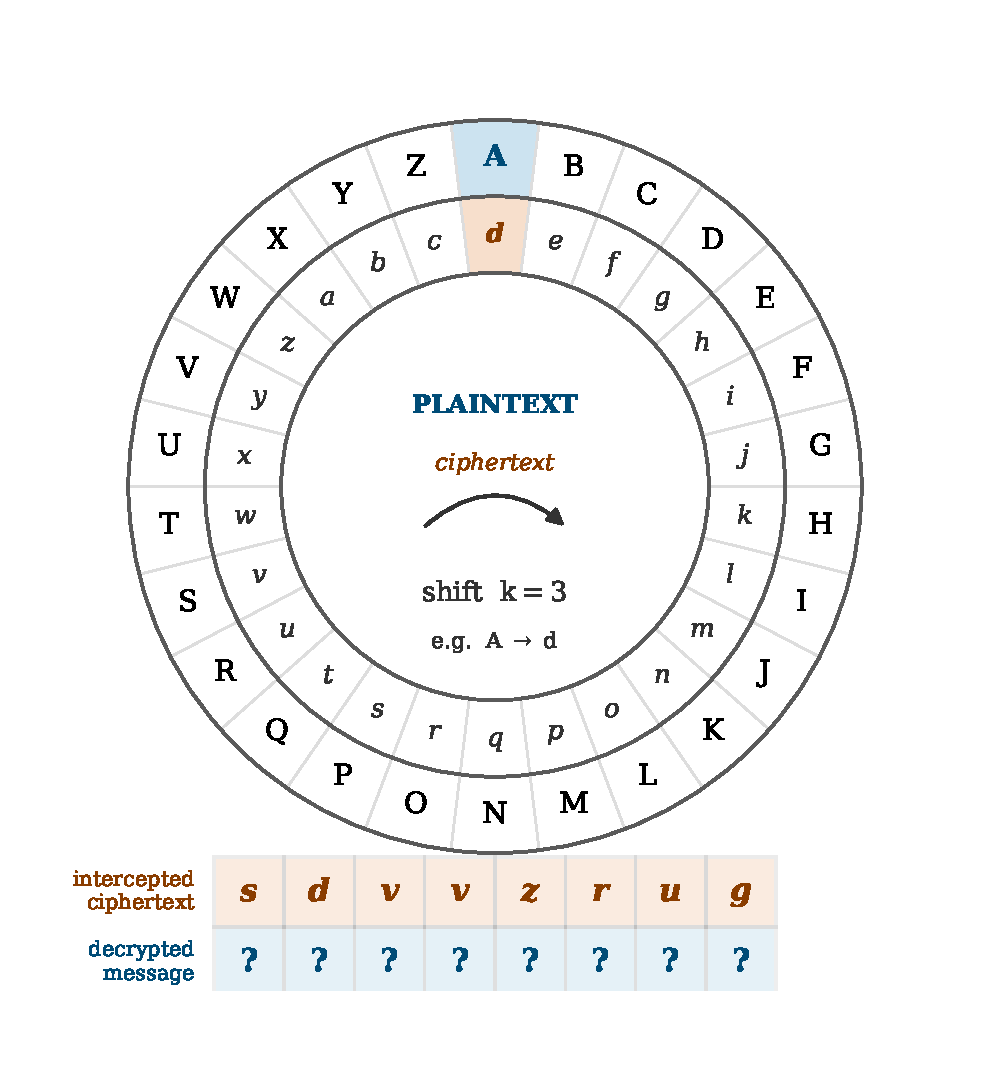
\includegraphics[width=0.62\textwidth]{figures/chapter1/caesar_cipher.pdf}
    \caption{The cipher disk used to encrypt and decrypt with the Caesar cipher.
    The secret key is simply the shift value $k$ (here $k = 3$). Encryption
    aligns the outer plaintext ring against the inner ciphertext ring, rotated by
    $k$ positions, and replaces each letter of the message with the one it meets
    on the inner ring; decryption is the inverse operation, reading from the inner
    ring back out. Formally, $E_k(x) = (x + k) \bmod 26$ and
    $D_k(y) = (y - k) \bmod 26$. The intercepted ciphertext below is left for the
    reader to recover. Its repeated letter already invites frequency analysis,
    and with only $25$ possible shifts the cipher is trivially brute-forced. A
    modern Advanced Encryption Standard (AES) cipher such as AES-256, by contrast, draws its key from
    $2^{256} \approx 10^{77}$ possibilities.}
    \label{fig:caesar_cipher}
\end{figure}

In the modern digital era, this dynamic stabilized around computational complexity. The bedrock of the internet, global commerce, and secure infrastructure rests on mathematical problems, such as factoring large integers or computing discrete logarithms, that are trivially easy to construct but practically impossible for classical computers to solve.

In late 1994, mathematician Peter Shor disrupted this equilibrium. He demonstrated that a hypothetical quantum computer could efficiently solve these exact mathematical problems, effectively neutralizing the public-key cryptography that secures modern communications~\cite{shor1994algorithms}.
A few weeks later, in January 1995, the author of this dissertation was born. The race was on.

\section{The Quantum Threat}

Over the intervening three decades, that theoretical result has evolved into a global engineering effort. Secure communication infrastructure is now entering a transition in which its foundational cryptographic assumptions can no longer be treated as stable design constants. The anticipated arrival of cryptographically relevant quantum computers (CRQCs) motivates a fundamental shift from classical public-key mechanisms toward two emerging technologies that will be explored in detail throughout this thesis: post-quantum cryptography (PQC) and quantum key distribution (QKD).

\subsection{Q-Day}

In security engineering, a \emph{zero-day} is a vulnerability that can be exploited before any defense exists, so that affected systems are compromised without prior warning. Q-Day is the cryptographic counterpart at global scale: the point at which a CRQC renders the public-key cryptography underpinning modern communication breakable, undermining not an individual system but a trust assumption common to nearly all of them simultaneously.

The exact date cannot be predicted. It depends on advances in scaling logical qubits and quantum error correction that have not yet been achieved, leading to a wide range of published timelines. More significant than any single estimate, however, is the consensus among the experts closest to the hardware. A CRQC within the next one to two decades is increasingly regarded as a realistic prospect rather than a remote one (Figure~\ref{fig:qday_timeline}). While individual forecasts vary, their collective trend is consistent.

Q-Day nevertheless differs from a conventional zero-day in one respect that is central to this dissertation: it is anticipated. Because the break is known in advance, the affected cryptography can be replaced before the capability matures, transforming a potentially abrupt failure into a planned, if time-constrained, migration.

\begin{figure}[htbp]
    \centering
    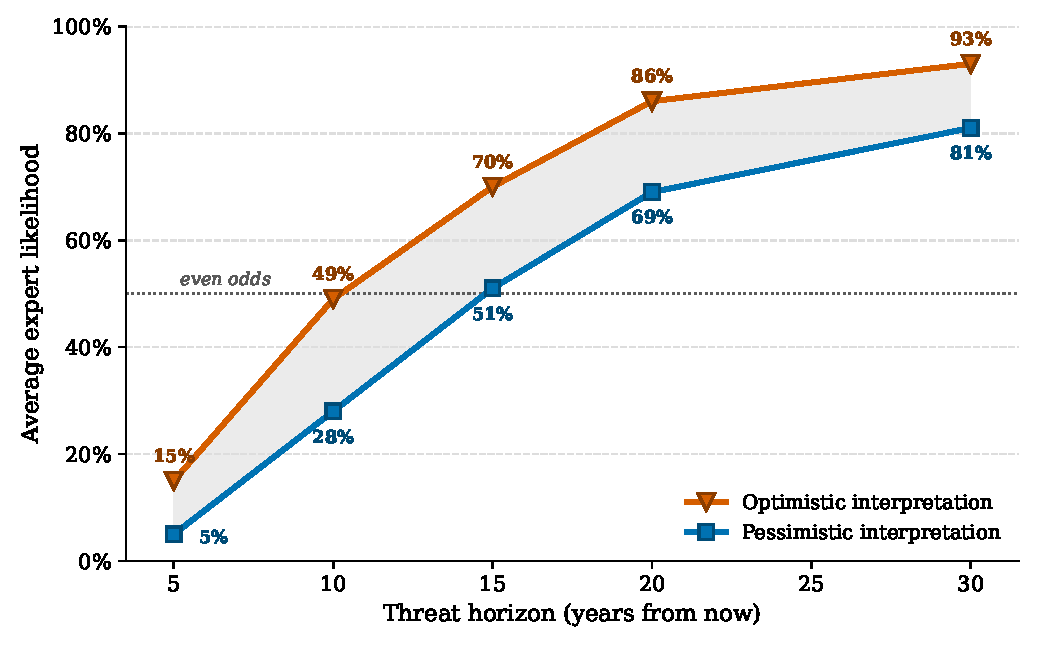
\includegraphics[width=0.8\textwidth]{figures/chapter1/qday_timeline.pdf}
    \caption{Averaged expert likelihood that a quantum computer able to break
    RSA-2048 within 24 hours will exist within a given horizon, under optimistic
    and pessimistic interpretations of the survey responses. Data
    from~\cite{mosca2026quantum}.}
    \label{fig:qday_timeline}
\end{figure}

\subsection{The Hardware Gap}

While the threat timeline is accelerating, a substantial gap remains between the state of the art in quantum hardware and the scale required for cryptanalysis. Breaking a standard 2048-bit RSA key using Shor's algorithm requires a fault-tolerant quantum computer capable of sustaining millions of operations. Historically, this was estimated to require around 20 million physical qubits~\cite{gidney2021factoring}.
However, recent algorithmic optimizations and architectural improvements, such as approximate residue arithmetic, magic state cultivation, and advanced quantum low-density parity check (qLDPC) codes, have drastically reduced these estimates. Current projections suggest that RSA-2048 could be factored in under a week using fewer than one million noisy physical qubits~\cite{gidney2025how}, and potentially under 100,000 physical qubits with next-generation qLDPC architectures~\cite{webster2026pinnacle}.

Despite these theoretical reductions, building a CRQC remains a monumental engineering challenge. As of 2026, gate-model superconducting processors have reached the order of one thousand physical qubits, with IBM's Condor processor featuring 1,121 superconducting qubits~\cite{ibmcondor2023}.
Other leading modalities have advanced in parallel: neutral-atom arrays from Atom Computing have crossed the 1,000-qubit milestone~\cite{atomcomputing2023}, while reconfigurable QuEra--Harvard arrays have demonstrated the first logical qubits at scale~\cite{bluvstein2024logical}.
Meanwhile, systems with lower physical qubit counts, such as Quantinuum's trapped-ion processors and Google's Willow chip, have focused on demonstrating high-fidelity operations and below-threshold error correction to create the first robust logical qubits~\cite{moses2023racetrack,googleqai2025below}.
Bridging the gap from today's hardware to the scale required for a CRQC necessitates solving complex control, cooling, and error-correction challenges.

It is important to stress that the achieved and required qubit counts are not directly comparable. The processors built to date consist of \emph{noisy} physical qubits, whereas the resource estimates above count the \emph{fault-tolerant} physical qubits needed once quantum error correction is layered on top, under idealized assumptions such as a physical error rate of $10^{-3}$ and microsecond-scale code cycles. The meaningful observation is therefore not a single headline ratio but the structural trend shown in Figure~\ref{fig:hardware_gap}: the estimated cost of breaking RSA-2048 has fallen by several orders of magnitude in little over a decade through algorithmic and error-correction advances, while hardware has scaled more slowly. The result is a hardware gap that remains large today but is being closed from both ends.

The rapid narrowing of this hardware margin has dismantled the consensus that infrastructure owners have decades to prepare. Just recently, the United States government slashed its original 2035 migration target~\cite{nsm10} by five years, mandating full post-quantum deployment across critical systems by 2030~\cite{eo14412,omb2026m2615}. This example shows that quantum resilience is no longer a gradual future upgrade, but an immediate infrastructure requirement. Consequently, the debate over \emph{whether} to adopt quantum-resilient cryptography is effectively settled; the primary engineering challenge is now \emph{how} to integrate these demanding new protocols into production networks before the hardware gap closes entirely.

\begin{figure}[htbp]
    \centering
    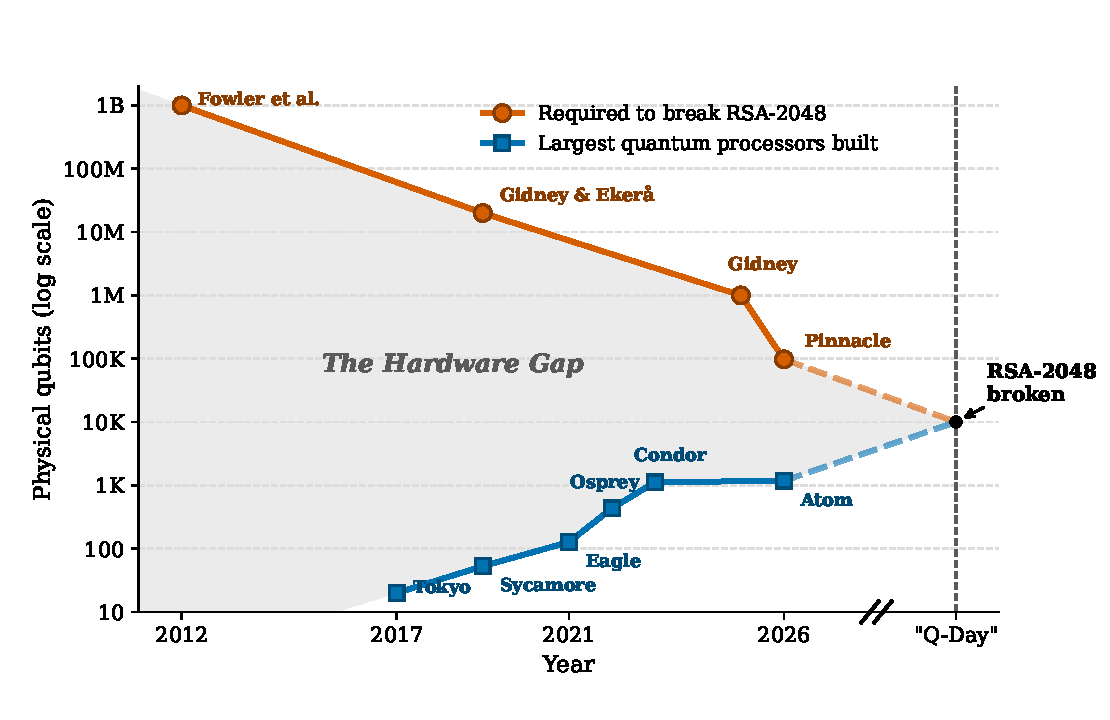
\includegraphics[width=0.85\textwidth]{figures/chapter1/hardware_gap.pdf}
    \caption{The hardware gap for factoring RSA-2048. The descending trend shows
    successive estimates of the physical qubits \emph{required} to factor a
    2048-bit RSA integer~\cite{fowler2012surface,gidney2021factoring,gidney2025how,webster2026pinnacle},
    while the ascending trend shows the largest gate-model quantum processors
    actually \emph{built}~\cite{arute2019quantum}. The two are not a like-for-like
    comparison: achieved counts are noisy physical qubits, whereas the required
    counts assume fault-tolerant physical qubits with error correction (physical
    error rate $\approx 10^{-3}$). The shaded region is the hardware gap, which has
    narrowed over time. To illustrate when this gap might close, the dashed lines show
    a stylized extrapolation towards a hypothetical ``Q-Day''.}
    \label{fig:hardware_gap}
\end{figure}

\subsection{The Dual Path to Quantum Resilience}

If a large-scale CRQC remains years away, why must communication infrastructure change today? The imperative is driven by ``Harvest Now, Decrypt Later'' (HNDL) attacks, where adversaries intercept and store encrypted traffic today, intending to decrypt it once quantum hardware matures~\cite{blanco2026practical}.

The urgency of this threat depends fundamentally on information value decay. Capturing, securely storing, and eventually processing petabytes of traffic on early fault-tolerant quantum computers will be astronomically expensive. Because not all secrets are created equal, this economic reality creates a natural divergence in how data must be protected. High-decay data, such as e-commerce transactions or session tokens, lose their value within minutes. By the time a CRQC is available, their residual value is effectively zero. In contrast, low-decay data, such as state secrets, genomic databases, or critical intellectual property, can retain immense value for decades, making them viable targets for long-term archiving today.

Defending against this threat relies on two fundamentally different paradigms: PQC and QKD.
PQC replaces vulnerable algorithms like RSA and elliptic curve cryptography with new computational problems, such as lattice- or hash-based cryptography, that are believed to be hard for both classical and quantum computers. Its primary advantage is scalability. PQC operates over existing classical networks. However, its security still rests on unproven mathematical assumptions. The unexpected collapse of candidate algorithms like SIKE highlights this risk~\cite{castryck2023sidh}. Building true confidence in new computational primitives requires years of intense cryptanalytic scrutiny.

In contrast, QKD offers information-theoretic security grounded in the laws of quantum mechanics. Because any attempt to eavesdrop on quantum states inevitably disturbs them, QKD provides a mathematically provable guarantee of secrecy that is immune to algorithmic breakthroughs or infinite computational power. While this theoretical guarantee is absolute, practical implementations remain vulnerable to hardware side-channels. Furthermore, its deployment comes at a steep practical cost. It requires specialized photonic hardware, dedicated optical channels, and complex control systems, making it difficult to scale.

Because data spans a vast spectrum of value and lifespan, a uniform defense is both economically and architecturally impractical. The massive volume of high-decay data requires the scalable deployability of PQC. Unconditionally high-value, low-decay secrets demand the eternal security of QKD. Between these poles, a protracted transition period requires crypto-agility and the flexible combination of multiple cryptographic mechanisms to hedge against potential algorithmic failures. Modern networks must therefore support a heterogeneous cryptographic ecosystem.

\section{Scope and Contributions}

\subsection{The Cross-Layer Imperative}

Recognizing the need for both PQC and QKD is only the first step; deploying them exposes a deeper architectural crisis. Neither solution can simply be dropped into existing systems as a software update.

PQC introduces significantly larger key sizes, heavier signatures, and complex arithmetic. When deployed at the scale of modern datacenters, these algorithms consume excessive CPU cycles and severely degrade network throughput and latency. Restoring performance requires pushing cryptographic operations out of the host processor and into specialized network infrastructure, such as data processing units (DPUs).

Similarly, scaling QKD beyond point-to-point physics experiments into operational infrastructure is an immense engineering challenge. It requires miniaturizing bulk optical components onto integrated photonic chips, designing high-throughput real-time post-processing pipelines to distill secure keys, and interfacing these quantum systems with classical network stacks.

Consequently, mitigating the quantum threat is not merely an algorithm selection problem---it is a fundamental integration challenge. A cryptographic primitive that is secure in theory is useless if it violates the latency, throughput, power, or observability constraints of the network. Scalable quantum-resilient communication therefore demands a \emph{cross-layer} approach, requiring systems to be co-designed across the device layer (integrated photonics and physical channels), the protocol layer (QKD post-processing and post-quantum algorithms), and the infrastructure layer (programmable networks, datacenter transport, and observability).

\subsection{The QUARC Project}

The work in this dissertation was carried out within Quantum Resistant
Communications: Advance Learning in Applied PQC Training (QUARC), a Marie
Sk\l{}odowska-Curie Actions (MSCA) doctoral network funded under Horizon Europe and run
as an industrial doctorate~\cite{QUARC2022,quarcwebsite}. QUARC was established to
train a cohort of doctoral researchers in the practical application of
post-quantum cryptography as the first standardized PQC algorithms moved from
specification toward real-world deployment, with each candidate spending a
substantial share of their time embedded within an industrial partner. For the
research reported here that partner was NVIDIA, and the work was shaped
throughout by close collaboration with its networking organization.

\subsection{Research Questions}

This dissertation is organized around the following research questions.

\begin{tcolorbox}[
    colback=gray!5!white,
    colframe=blue!50!black,
    title=\textbf{Research Questions (RQs)},
    fonttitle=\bfseries,
    sharp corners,
    boxrule=0.8pt]
\begin{enumerate}[label=\textbf{RQ\arabic*:}, leftmargin=1.2cm]
    \item How can PQC workloads be accelerated and
deployed efficiently on programmable network infrastructure?
    \item What architectural choices make QKD systems more scalable and
practical in high-performance datacenter networks?
    \item How can integrated photonic entanglement sources be designed and
characterized for deployable, wavelength-division multiplexed QKD systems?
    \item How do device-level, protocol-level, and infrastructure-level design
choices interact when building scalable quantum-resilient communication
systems?
\end{enumerate}
\label{en:researchquestions}
\end{tcolorbox}

RQ1--RQ3 address three complementary engineering problems: deploying PQC
efficiently, scaling QKD systems, and designing deployable integrated quantum
sources. RQ4 provides the cross-layer synthesis by examining how decisions in
one area constrain or enable the others.

\subsection{Publications and Intellectual Property}

The main body of this dissertation is organized around published manuscripts,
as well as manuscripts currently under review, produced during this PhD.
In addition to these peer-reviewed publications and submissions, the industrial
research undertaken within the QUARC project yielded several patent applications.
While the full technical details of these patents are omitted due to intellectual
property restrictions, their scope maps directly to the focus of this thesis,
and their conceptual role in the overarching architecture is mapped in
Figure~\ref{fig:field-venn}. A complete list of the publications (P1--P9) and
inventions (I1--I4) can be found in the List of Publications.

\section{Structure}

The structure of the dissertation is as follows:

\medskip
\textbf{Chapter~\ref{ch:background}} establishes the cross-layer framework used throughout the dissertation and introduces the DPU as a recurring infrastructure substrate for the offload and observability contributions. Topic-specific background is developed in each paper-centric chapter where it is needed.

\medskip
The core contributions are then divided into three parts:

\medskip
\textbf{Part~I --- Quantum Key Distribution} treats quantum key distribution as a deployable network capability rather than only a point-to-point protocol.
\begin{itemize}
\item \textbf{Chapter~\ref{ch:quantum-sources}} discusses the integrated photonic foundations of practical quantum-secure networking, addresses RQ3, and presents P1 and P2.
\item \textbf{Chapter~\ref{ch:qkd-dpu}} discusses scalable QKD post-processing offload on programmable network hardware, addresses RQ2, and presents P3.
\end{itemize}

\medskip
\textbf{Part~II --- Post-Quantum Cryptography} investigates how post-quantum cryptographic algorithms can be executed efficiently on heterogeneous platforms, collectively addressing RQ1.
\begin{itemize}
\item \textbf{Chapter~\ref{ch:dpu-pqc}} discusses CPU-GPU-DPU workload partitioning and latency tradeoffs for datacenter-scale PQC deployment, addresses RQ1, and presents P4 and P5.
\item \textbf{Chapter~\ref{ch:ai-pipelines}} discusses the application of post-quantum mechanisms to secure end-to-end artificial intelligence (AI) pipelines, addresses RQ1, and presents P6.
\end{itemize}

\medskip
\textbf{Part~III --- Datacenter-Scale Security} widens the lens from individual devices and nodes to the datacenter operating as a whole, and stops treating the shared substrate beneath it as a trustworthy given. It examines that substrate first as an attack surface and then as a defensive vantage point, exposing the cross-layer interactions at the heart of RQ4.
\begin{itemize}
\item \textbf{Chapter~\ref{ch:rdma}} treats the infrastructure as an attack surface, spanning device-level side channels through to the ordering- and timing-related risks of remote direct memory access (RDMA) over high-throughput optical fabrics, addresses RQ4, and presents P7.
\item \textbf{Chapter~\ref{ch:confidential-ai}} inverts that argument into a defence, using cross-layer observability and intrusion detection to protect confidential AI training clusters, addresses RQ4, and presents P8 and P9.
\end{itemize}

\medskip
Finally, \textbf{Chapter~\ref{ch:cross-layer}} synthesizes the cross-layer lessons from the preceding parts to fully resolve RQ4, discussing limitations and the future outlook.

\medskip
While this structure divides the thesis sequentially by technological domain, scalable quantum-resilient communication is an inherently cross-layer challenge. As illustrated in Figure~\ref{fig:field-venn}, these domains are highly entangled in practice. The pairwise overlaps mark where QKD and PQC integrate directly with programmable network hardware, while a multi-hybrid key-exchange architecture draws on all three parts simultaneously.

\begin{figure}[htbp]
    \centering
    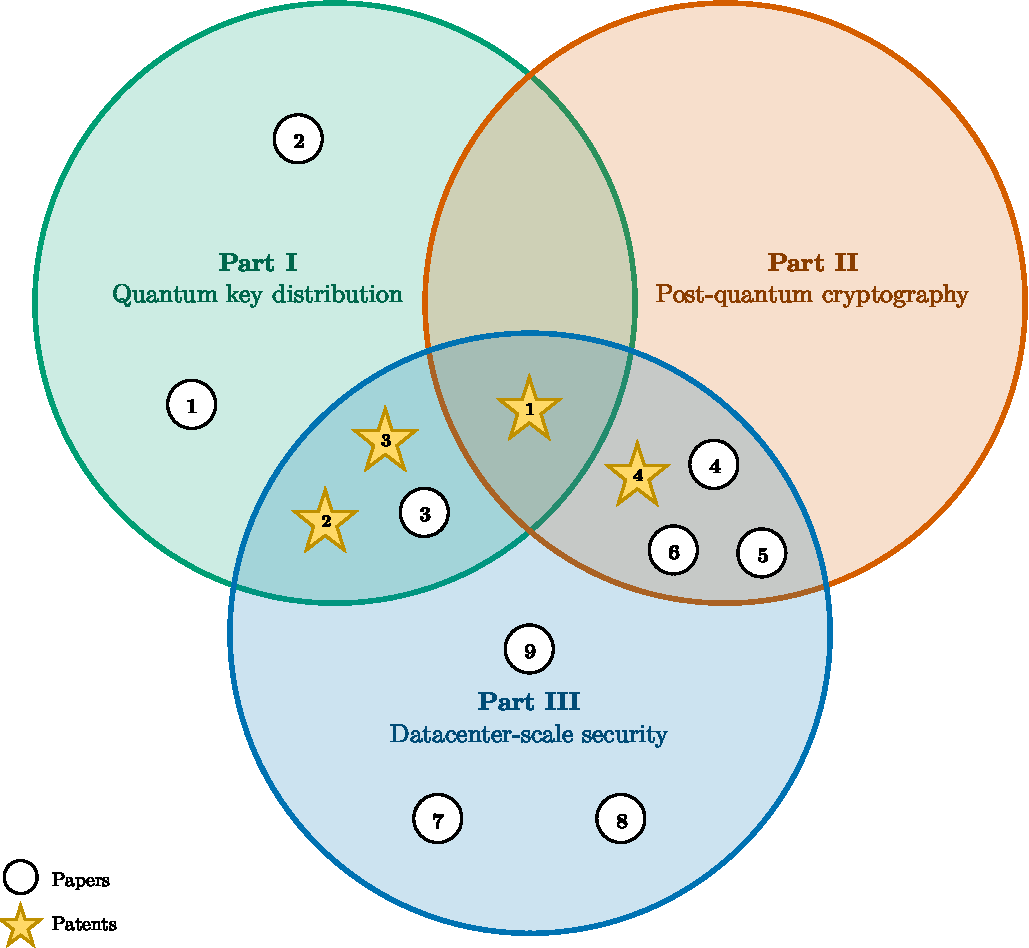
\includegraphics[width=0.7\textwidth]{figures/chapter1/field_venn.pdf}

    \caption{Mapping of the dissertation's contributions onto its three core
    parts. Circular markers denote peer-reviewed papers and star markers denote
    patents.}
    \label{fig:field-venn}
\end{figure}

\chapter{The Cross-Layer Approach and the DPU Substrate}
\label{ch:background}

In 2010, a group of researchers eavesdropped on a commercial QKD link and read
the secret key in full, without leaving a trace
in the error rate that was supposed to expose them. 
They did not exploit a fault in the photonic devices, nor did they find a vulnerability in the
QKD protocol. 
Instead, they shone a continuous beam of bright light
into the receiver, driving its single-photon detectors out of their quantum
regime and into a classical mode in which they responded only to a sharp spike of
power. From that point on, the attacker could decide exactly when each detector
``clicked'' and thereby dictate the key the two endpoints believed they had shared
in secret~\cite{lydersen2010hacking}.
The mathematics was untouched and the hardware behaved exactly as it was built to.
The weakness lived in the seam between them: a silent assumption the protocol layer
made about the device layer---that a single-photon detector responds to light the
way its idealized model says it does. Examined on its own terms, neither layer was
at fault. The vulnerability existed only at their boundary, where one layer's proof
met the other's physics.

This episode is a small parable for the argument of this dissertation. The
exploitable weakness belonged to no single layer; it emerged where they met, at an
interface whose assumptions no one had thought to test. A guarantee established at
one layer of a secure system is only as strong as what it takes for granted about
the layers above and below it---and it is at those boundaries, rather than within
any one layer, that security tends to fail. The paper-centric chapters that follow span photonic devices, quantum-key
post-processing, post-quantum cryptographic acceleration, datacenter transport,
and security observability. Read individually, they appear to belong to separate
research communities, each with its own models, metrics, and implicit assumptions.
Two things make them a single dissertation: a shared \emph{method}---a cross-layer
view of secure communication in which a design choice at one layer is judged by its
consequences at the others---and a shared \emph{substrate}---the data processing
unit (DPU) on which nearly every contribution is built or observed.

This chapter establishes only those two common threads. It first sets out the
cross-layer lens and the analytical method that recur throughout the thesis, and
then introduces the DPU as the hardware that connects cryptographic primitives to
the infrastructure. The technical background specific to each topic---integrated
photonic sources, QKD post-processing, post-quantum primitives, RDMA fabrics, and
confidential computing---is deliberately deferred to the chapter that needs it,
where it can be developed alongside the corresponding contribution. The cross-layer
dependencies that emerge once all of these pieces are in place are revisited and
resolved in Chapter~\ref{ch:cross-layer}.

\section{The Cross-Layer Security Stack}
\label{sec:bg-stack}

The introduction framed the quantum threat not merely as an algorithm-selection
problem, but as a systemic architectural challenge governed by the boundaries
between the device, protocol, and infrastructure layers. Information value decay
explains \emph{which} protection each class of traffic warrants rather than why the
problem is cross-layer: unconditionally high-value, slowly decaying secrets justify
the deployment complexity and bespoke hardware of physics-based security, primarily
QKD, which offers information-theoretic security that is immune to algorithmic
advances, while the much larger volume of computationally protected, rapidly
decaying traffic is served by PQC, which must operate at datacenter scale. What
makes the problem cross-layer is that both physics-based and computationally-based
protections must ultimately run on the same programmable network fabric, where
their device- and protocol-level guarantees collide with one shared set of
infrastructure constraints.

To analyze this heterogeneous landscape, this dissertation structures the response
along three distinct but interacting layers, illustrated in Figure~\ref{fig:cross_layer_stack}.

\begin{figure}[htbp]
    \centering
    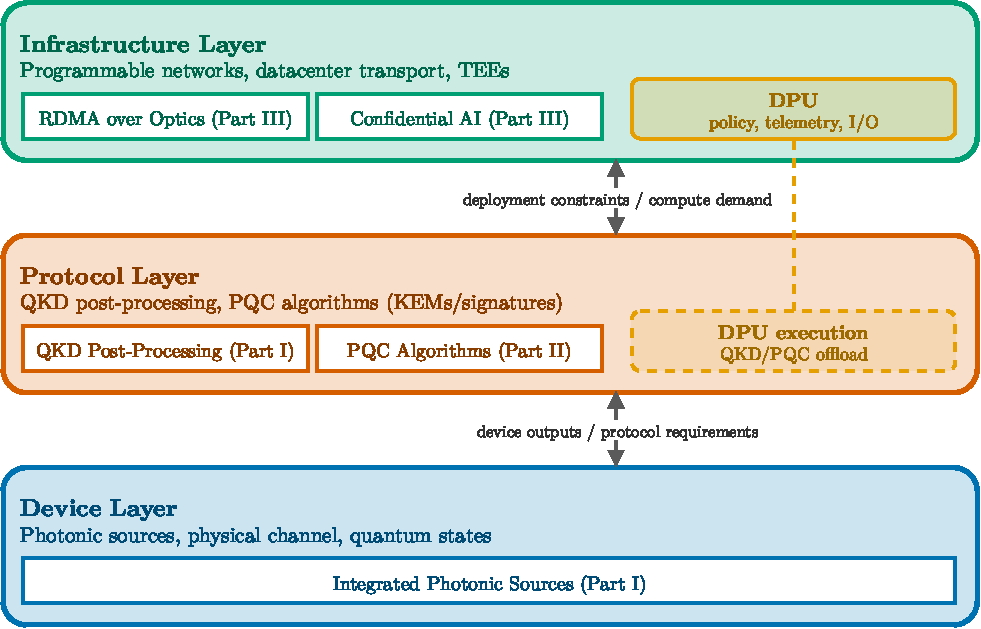
\includegraphics[width=0.85\textwidth]{figures/chapter2/cross_layer_stack.pdf}
    \caption{The cross-layer security stack investigated in this dissertation. The device layer supplies physical resources; the protocol layer consumes those resources to produce key material and authenticated channels; the infrastructure layer determines deployment viability. The Data Processing Unit (DPU) serves as both the execution substrate and observation point spanning the upper layers.}
    \label{fig:cross_layer_stack}
\end{figure}

\begin{itemize}
  \item a \textbf{device layer}, where photonic sources and the physical channel
        determine the quality and stability of the quantum states that security
        protocols can assume. The governing quantities here are physical: spectral
        purity, free spectral range (FSR), quality factors, and loss budgets.
  \item a \textbf{protocol layer}, where QKD post-processing and post-quantum
        algorithms turn raw physical or mathematical resources into usable key
        material and authenticated channels. The governing quantities here are
        algorithmic and informational: key distillation rates, security margins,
        computational complexity, and message sizes.
  \item an \textbf{infrastructure layer}, where programmable network hardware,
        datacenter transport, and confidential-computing environments decide
        whether those protocols can actually be deployed, accelerated, observed,
        and defended at scale. The governing quantities here are operational:
        latency, throughput, determinism, queue depth, and observability.
\end{itemize}

\subsection{The Cross-Layer Method}

The recurring method of the thesis is to take a security or performance
assumption stated at one layer and test what happens to it when it is mapped
onto another. An isolationist view often hides systemic vulnerabilities. For
instance, a protocol proof might assume perfect single-photon sources, while the
device layer actually exposes multiphoton states subject to thermal drift. A
post-quantum signature scheme might be highly efficient when benchmarked on a
single idle core, but its tail latency might collapse under heavy datacenter
batching. A transport layer might be provably encrypted by MACsec or IPsec, yet
still leak critical application state through traffic ordering and timing behavior.
Finally, an infrastructure defender operating a confidential-computing cluster must
detect intrusions without seeing the payload, violating the assumptions of classical
intrusion detection systems.

Research questions RQ1--RQ3 each target a single layer---PQC deployment, QKD
architecture, and photonic-source design---while RQ4 binds them by exposing
exactly these cross-layer failure modes.

\section{Programmable Network Infrastructure for Security Offload}
\label{sec:bg-dpu}

The single piece of hardware common to nearly every contribution in this thesis is
the DPU. It is introduced here, once, because it underpins the QKD, PQC, and
infrastructure chapters alike.

SmartNICs and DPUs represent a paradigm shift in datacenter architecture. They extend
the network interface from a passive I/O endpoint---responsible only for moving packets
between the wire and host memory---into an active, programmable execution environment.
In modern DPU architectures like the NVIDIA BlueField series, the device features a
cluster of general-purpose Arm CPU cores, dedicated hardware accelerators (including
inline cryptographic engines for AES-GCM and public-key acceleration), substantial
on-board memory, and programmable packet-processing pipelines~\cite{burstein2021nvidia}.
In more advanced configurations, DPUs provide direct GPU-connected datapaths (e.g.,
GPUDirect remote direct memory access, RDMA) that bypass the host CPU entirely
(Figure~\ref{fig:dpu_architecture}).

\begin{figure}[htbp]
    \centering
    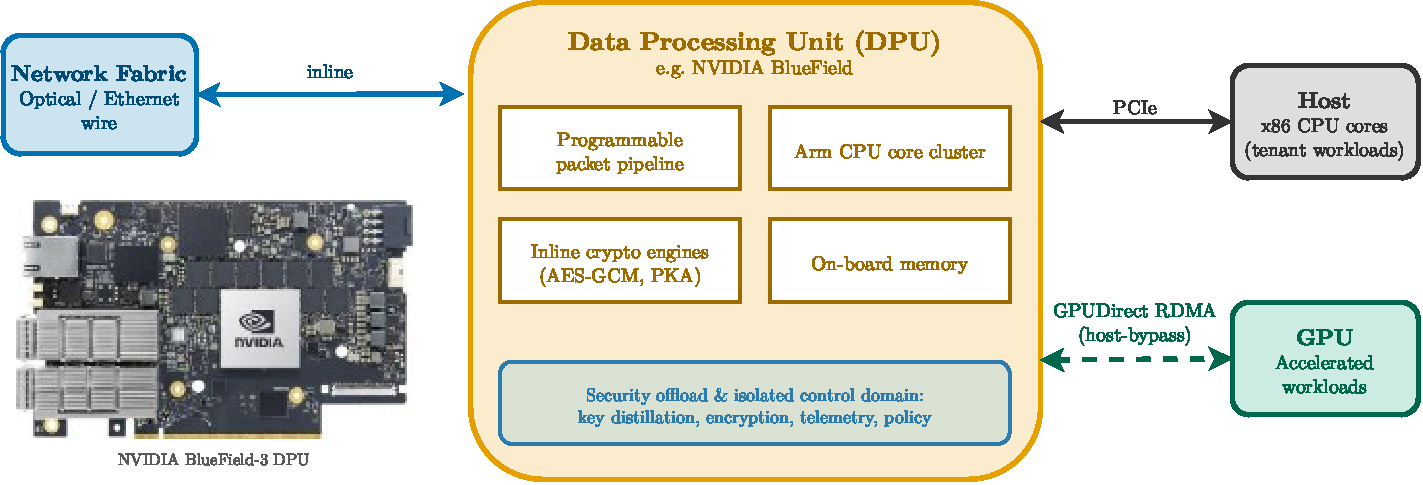
\includegraphics[width=0.95\textwidth]{figures/chapter2/dpu_architecture.pdf}
    \caption{The DPU as an execution substrate and observation point. Sitting
    inline between the network fabric and the host, the DPU couples a programmable
    packet pipeline, an Arm CPU core cluster, inline cryptographic engines, and
    on-board memory. Security-critical functions are offloaded into this isolated
    control domain, while a GPUDirect RDMA datapath moves data to the GPU without
    traversing the host CPU.}
    \label{fig:dpu_architecture}
\end{figure}

This architecture makes it possible to place security-critical operations---such as
key distillation, cryptographic encapsulation, storage encryption, telemetry collection,
and firewall policy enforcement---at the edge of the host rather than deep inside its
operating system~\cite{meyer2026hqc}. By moving these functions to the DPU, the host CPU
is freed to run tenant workloads, and the infrastructure provider retains a secure,
isolated domain to enforce policies even if the host is compromised.

\subsection{The Offload Decision Framework}

However, offload is not automatically beneficial. Moving a task from a powerful,
high-frequency x86 host CPU to a lower-power Arm core on a DPU introduces significant
overheads: data movement across the PCIe bus, queueing delays, synchronization locks,
resource contention among DPU cores, and additional software complexity. The host CPU
will almost always win a raw single-thread benchmark.

Therefore, the useful question is never whether a DPU is ``faster'' in isolation. The
relevant architectural questions are:
\begin{enumerate}
    \item \textbf{Partitioning:} Which specific part of a pipeline should move to the DPU?
    \item \textbf{Batching:} Under what traffic conditions and batch sizes does the offload break even?
    \item \textbf{Bottlenecks:} What becomes the new system bottleneck once the compute task has moved?
    \item \textbf{Determinism:} How stable is the latency distribution under heavy, concurrent load?
\end{enumerate}

These questions recur in identical form across different domains in this thesis. They
dictate how QKD post-processing scales (Chapter~\ref{ch:qkd-dpu}), whether post-quantum
key encapsulation meets handshake latency budgets (Chapter~\ref{ch:dpu-pqc}), and how
secured end-to-end AI pipelines manage image I/O (Chapter~\ref{ch:ai-pipelines}). For this reason,
the DPU is treated here as a unifying substrate rather than as a detail of any single
chapter.

Furthermore, the same programmability that enables offload also transforms the DPU into
a natural observation point. Placed inline between the network and the host, the DPU
can inspect traffic metadata, connection timing, and queue depths without host interference,
a capability that becomes the foundation of the confidential-AI observability discussed
in Chapter~\ref{ch:confidential-ai}.


\part{Quantum Key Distribution}
\label{part:qkd}

\chapter{Integrated Quantum Sources for Quantum Networks}
\label{ch:quantum-sources}

\section{From Photonic Devices to Network Components}

Quantum-secured networks depend on physical devices whose behavior must remain predictable after they leave a controlled laboratory setting. To build a robust quantum network, we must bridge the gap between idealized cryptographic protocols and the imperfect physical reality of the devices that implement them. Entangled-photon sources are one such foundational device class: they determine the spectral structure, brightness, purity, and long-term stability of the quantum states that later protocols consume. If these source properties drift with fabrication tolerances, thermal changes, or uncontrolled mode interactions, then the network layer inherits an unstable security and performance foundation.

This chapter begins the thesis body at the photonic-device layer. It examines dual-coupled micro-ring resonators as integrated sources for frequency-bin entangled photons. The common thesis-level question is not only whether such a device can generate useful quantum states, but whether it can be designed, tuned, and modeled in a way that makes it suitable for larger quantum--classical network systems.

\paragraph{Scope and assumptions.} This dissertation is a systems and networking contribution rather than a study of quantum-mechanical foundations. It assumes familiarity with the basic formalism of quantum states, measurement, entanglement, and the no-cloning theorem, and treats these as building blocks instead of deriving them; readers seeking that background are referred to standard texts~\cite{nielsen2010quantum}. For a deeper exploration of quantum optics, particularly concerning spatial modes and free-space optical communication, readers are referred to the author's prior work~\cite{meyer2024master}. The contributions reported here lie in how these primitives are designed, accelerated, stabilized, and integrated across the device, protocol, and infrastructure layers.

\section{Nonlinear Optics and Four-Wave Mixing}
\label{sec:qsrc-nonlinear}

The generation of entangled photon pairs in integrated photonics relies fundamentally on nonlinear optical processes. In centrosymmetric materials such as silicon and silicon nitride, the lowest-order nonlinear response is the third-order susceptibility, $\chi^{(3)}$. This nonlinearity mediates spontaneous four-wave mixing (SFWM), the process by which two pump photons are annihilated to create a signal and an idler photon pair.

Energy conservation dictates that the frequencies of the generated photons satisfy $2\omega_p = \omega_s + \omega_i$, where $\omega_p, \omega_s$, and $\omega_i$ are the pump, signal, and idler frequencies, respectively. Momentum conservation, or phase matching, requires that the propagation constants satisfy $2k_p = k_s + k_i + \Delta k$, where $\Delta k$ is the phase mismatch. In a microring resonator, phase matching is naturally achieved when the pump, signal, and idler fields align with the cavity resonances.

The efficiency of SFWM is highly dependent on the spatial overlap of the optical modes within the waveguide and the nonlinear refractive index of the material. Silicon nitride ($\text{Si}_3\text{N}_4$) has emerged as a leading platform for SFWM due to its ultra-low linear propagation loss, wide transparency window spanning from the visible to the mid-infrared, and absence of two-photon absorption at telecom wavelengths. These properties allow for the use of high-power continuous-wave pumps, maximizing the pair generation rate while maintaining high spectral purity.

By carefully engineering the waveguide cross-section, the group velocity dispersion (GVD) can be tailored to ensure broad phase-matching bandwidths. This dispersion engineering is critical for generating frequency-bin entangled states, where the signal and idler photons can occupy multiple pairs of symmetric resonance modes, creating a high-dimensional entangled state suitable for multiplexed quantum communication.

\section{Microring Entanglement Sources}
\label{sec:qsrc-microring}

Integrated photonics addresses the device-level bottleneck in deployable quantum
communication. Traditional tabletop optics, with discrete non-linear crystals and
mirrors, are too fragile, bulky, and expensive for wide-scale deployment. Photonic
integrated circuits (PICs) aim to miniaturize these components onto a semiconductor
chip using fabrication processes compatible with existing CMOS or telecom infrastructure.

For entanglement-based QKD and future repeater networks, the photon source is the critical component. It determines
the spectral structure, brightness, purity, and long-term stability of the photon pairs
that every subsequent protocol stage consumes~\cite{Wehner2018}. If a source emits
multiphoton pulses or indistinguishable spectral modes drift due to temperature fluctuations,
the visibility of quantum interference drops, the QBER rises,
and the protocol may fail to generate secure keys.

The work in this chapter focuses on microring resonators as candidate sources for
frequency-bin entanglement via spontaneous four-wave mixing (SFWM). In a microring,
light circulates and interferes constructively only at specific resonant frequencies
separated by the free spectral range (FSR). Key physics and engineering considerations
include:

\begin{itemize}
    \item \textbf{Quality Factor ($Q$):} A measure of the resonator's photon lifetime.
    High-$Q$ rings generate highly coherent, narrow-linewidth photons but are extremely
    sensitive to fabrication variations and thermal drift.
    \item \textbf{Thermal Tuning and Stability:} Refractive indices are temperature-dependent.
    Maintaining precise alignment with standardized telecom grids requires continuous,
    active thermal tuning, which can inadvertently affect the FSR and disrupt entanglement symmetry.
    \item \textbf{Spectral Purity (Schmidt Number):} A mathematically pure bipartite entangled
    state has a Schmidt number of 1. Real sources suffer from spectral correlations
    that degrade purity, necessitating precise dispersion engineering or tight filtering.
    \item \textbf{Platform Tradeoffs:} Silicon nitride ($\text{Si}_3\text{N}_4$) offers ultra-low
    loss and broad transparency but lacks the strong electro-optic (Pockels) effect of
    lithium niobate ($\text{LiNbO}_3$), meaning the choice of material dictates the tuning mechanisms
    available~\cite{Kumar2015,Mao2018,Grebenchukov2023}.
\end{itemize}

To provide the precise control required for networking, the dual-coupled architecture adds an auxiliary resonator to the main photon-pair generation ring. This additional degree of freedom can be used to reshape the spectral response of the source, compensate for nonidealities, and expose a control interface between device physics and network-facing metrics such as channel spacing, heralded purity, and Schmidt number. In this sense, the chapter treats source engineering as the first cross-layer problem of the dissertation: a physical-layer design choice must be made legible to the network and security layers built above it.

These device-derived quantities are precisely the parameters that determine the budget
available for coexistence with classical traffic. They define the point at which the
device layer becomes legible to the network layer above it.

\section{Source Characterization and Network Metrics}
\label{sec:qsrc-characterization}

Before an integrated quantum source can be deployed in a network, its performance must be quantified using metrics that translate directly to cryptographic utility. The raw generation rate of photon pairs is insufficient on its own; the quality of the entanglement and the distinguishability of the photons from background noise are paramount.

The primary figure of merit for the signal-to-noise ratio of a photon-pair source is the Coincidence-to-Accidental Ratio (CAR). It compares the rate of true coincident detection events (where both the signal and idler photons from a single pair are detected) to accidental coincidences (caused by dark counts, detector jitter, or uncorrelated photons from multi-pair emission). A high CAR is essential for maintaining a low quantum bit error rate (QBER) in the subsequent QKD protocol.

Another critical metric is the heralded single-photon purity. In entanglement-based protocols, the detection of an idler photon "heralds" the presence of the signal photon. If the source suffers from strong spectral correlations between the signal and idler, the heralded state will be mixed rather than pure, degrading the visibility of two-photon interference (such as the Hong-Ou-Mandel effect). The Schmidt number quantifies this purity: a Schmidt number of $1$ indicates a perfectly factorable, pure state. Dispersion engineering in microrings, as discussed in Section~\ref{sec:qsrc-nonlinear}, aims to minimize these correlations to approach ideal purity.

\section{Distance Scaling and Quantum Repeaters}
\label{sec:qsrc-distance}

While point-to-point QKD has been demonstrated over hundreds of kilometers, it faces a fundamental scaling limit. In classical optical networks, the exponential attenuation of light in standard telecom fiber is overcome using optical amplifiers (such as erbium-doped fiber amplifiers, or EDFAs) spaced every 80 to 100 kilometers. However, the no-cloning theorem strictly forbids the deterministic amplification of unknown quantum states. 

As a result, the key rate in a direct QKD link decays exponentially with distance. While state-of-the-art techniques like Twin-Field QKD (TF-QKD)~\cite{lucamarini2018overcoming} have pushed the maximum transmission distance past 800 kilometers~\cite{wang2022twinfield}, the resulting secure key rates at these extreme distances are often on the order of bits per second---insufficient for encrypting high-volume datacenter traffic. Figure~\ref{fig:qkd-distance-rate} summarizes this distance--rate tradeoff: state-of-the-art demonstrations cluster below the repeaterless bound, and only quantum repeaters restore favourable scaling at long distance.

\begin{figure}[htbp]
  \centering
  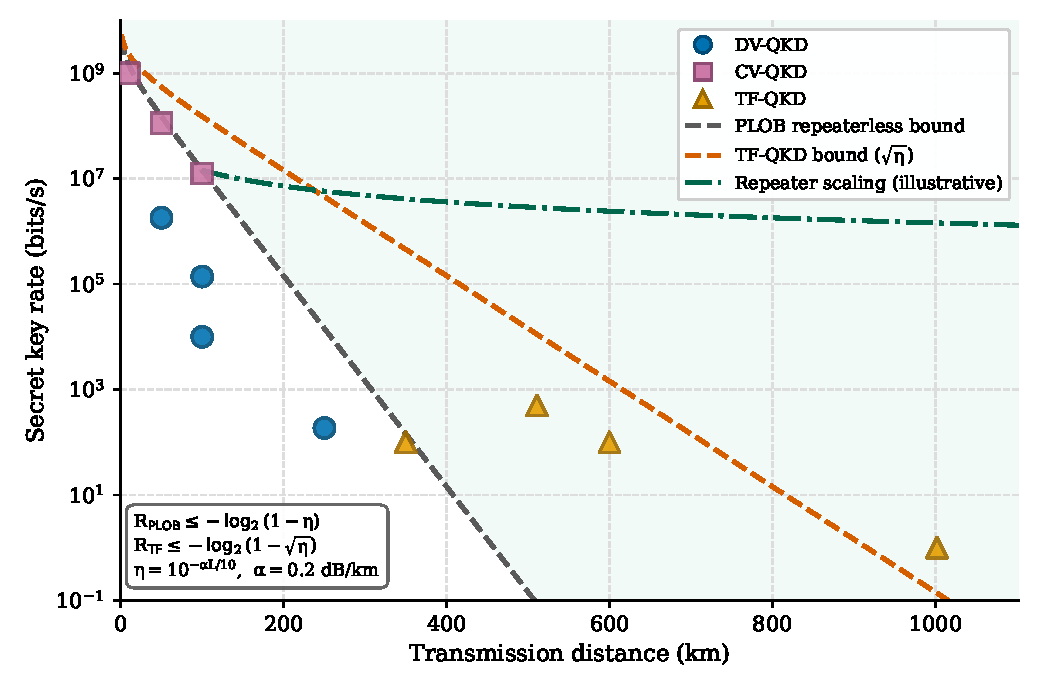
\includegraphics[width=\linewidth]{figures/chapter3/distance_keyrate.pdf}
  \caption[Distance scaling of QKD secret key rate]{Secret key rate as a
  function of transmission distance for quantum key distribution. In a direct,
  repeaterless link the secret key rate is fundamentally limited by the
  repeaterless Pirandola--Laurenza--Ottaviani--Banchi (PLOB)
  bound~\cite{pirandola2017fundamental} (grey dashed) and decays exponentially
  with distance.
  Twin-Field QKD improves the asymptotic scaling to $\sqrt{\eta}$ (vermillion
  dashed), extending reach beyond $1000$~km but only at rates of order bits per
  second. Restoring favourable, polynomial scaling at long distance requires
  quantum repeaters (green dash--dot, illustrative schematic), which lift the
  achievable rate into the shaded region above the PLOB bound. Markers show
  state-of-the-art WDM-compatible demonstrations (DV-, CV- and
  TF-QKD)~\cite{wang2025highrate,dynes2016ultrahigh,dolphin2023hybrid,ribezzo2023underwater,chen2021twinfield511,pittaluga2021repeaterlike,liu2023experimental1000,zhou2023twinfield};
  all lie below or near the repeaterless bound. Bounds assume standard $0.2$~dB/km fibre
  and a $1$~GHz reference clock; the repeater curve is illustrative, not
  measured.}
  \label{fig:qkd-distance-rate}
\end{figure}

To overcome this distance-rate tradeoff and achieve polynomial scaling, a global quantum network requires \emph{quantum repeaters}~\cite{briegel1998quantum}. Quantum repeaters divide a long-distance link into shorter, manageable segments. They operate by establishing entanglement across each short segment and then using entanglement swapping (a joint Bell-state measurement) to stitch these segments together, effectively teleporting the entanglement to the endpoints. 

The realization of quantum repeaters relies heavily on two components: quantum memories to store states until adjacent links succeed, and highly efficient, scalable sources of entangled photons to continuously populate the links. This necessity places immense pressure on the design of the photon sources: they must be bright, deterministic (or highly multiplexed), and spectrally compatible with the optical fibers carrying them.

\section{Coexistence with Classical Infrastructure}
\label{sec:qsrc-coexistence}

A further challenge for deploying quantum networks is the economic unfeasibility of laying dedicated ``dark fiber'' exclusively for quantum traffic. Practical quantum networking must co-exist with classical optical communications on the same fiber infrastructure using Wavelength Division Multiplexing (WDM). 

Integrating single-photon quantum channels alongside classical channels carrying milliwatts of power is notoriously difficult. The primary obstacle is spontaneous Raman scattering: the intense classical lasers scatter photons across a broad spectrum within the fiber, creating a noise floor that easily overwhelms the fragile quantum signals.

Overcoming Raman noise and achieving coexistence requires precise spectral filtering and alignment with the ITU telecom grid. The entangled photon sources must generate narrow-linewidth states at specific, standardized frequencies, and their emission characteristics must remain perfectly stable over time to allow ultra-tight filtering at the receiver. This requirement elevates the photon source from a physics experiment to a highly constrained network engineering component.

\section{Mapping Device Physics to Network Security}

The work in this chapter is written around the following mapping between low-level device behavior and the network requirements introduced in Chapter~\ref{ch:background}:

\begin{itemize}
  \item It addresses how quantum-secure networking primitives can be made compatible with deployed optical infrastructure. The focus is on C-band, wavelength-division-multiplexed operation and on resonator behavior that can be related to telecom channel plans~\cite{Kumar2015,Mao2018}.
  \item It addresses how low-level device parameters become system-level security constraints. Spectral purity, free spectral range stability, and the Schmidt number are device-derived quantities, but they influence interference visibility, quantum-bit error rate, and the practical budget available for coexistence with classical traffic~\cite{Grebenchukov2023}.
  \item It introduces the thesis pattern of cross-layer abstraction. Rather than treating a quantum source as a black box, the chapter asks which control variables and models are needed before a source can be used as a predictable component in a quantum network.
\end{itemize}

This chapter also sets up the transition to programmable network infrastructure in Chapter~\ref{ch:qkd-dpu}. The quantum source provides the raw optical resource, while later chapters ask how the resulting key material, cryptographic work, and observability tasks can be handled by DPUs, SmartNICs, and datacenter network systems.

\section{Contribution and Articles}

This chapter is built around two contributions that, taken together, move the dual-coupled microring (DCM) source from a promising integrated-photonics component toward a predictable network-engineering object. The author contributed to connecting the device studies to network requirements, the simulation-driven evaluation, and the thesis-level system interpretation; the experimental device work, modeling, and supervision were collaborative efforts with the co-authors.

The first contribution (P1), \enquote{Simulation-Driven Optimization of Dual-Coupled Micro-Ring Entanglement Sources for Quantum Optical Networks}, accepted to the 26th International Conference on Transparent Optical Networks (ICTON 2026), establishes the theoretical and modeling foundation for the chapter. It presents a coupled-mode-theory digital twin for the DCM source, relating auxiliary-cavity detuning, inter-ring coupling, and dispersion to photon-pair purity, brightness, and Schmidt number. By mapping low-level physical parameters to network-facing metrics, it defines the optimization space required to engineer quantum sources for specific network applications.

The second contribution (P2), \enquote{Free Spectral Range Stability under Linear Thermal Tuning in a Dual-Coupled Microring Resonator}, presented at the 2026 International Conference on Science and Electrical Engineering (ICSEE), provides the experimental validation of the device's stability. While the first paper demonstrated how the source can be optimized in simulation, this work grounds those findings in physical reality. Its key role is to show that thermal tuning of the auxiliary resonator---a necessary control mechanism---preserves the predictable free spectral range behavior required for channelized quantum network operation.

Together, the two papers establish that source behavior can be modeled, optimized, and physically stabilized in terms that later network layers can consume. This matters because quantum-secure communication is often limited by interfaces between layers: physical devices expose imperfect states; protocols assume idealized state properties; network planners allocate wavelengths and power budgets; and operators need stable, remotely configurable behavior. The resulting thesis claim is deliberately bounded. The chapter does not demonstrate a complete deployed quantum network, nor does it by itself close the practical-security gap of QKD systems; it establishes a modelable, stabilizable source as the foundation on which the rest of the thesis builds.

Two limitations should remain visible in the final dissertation. First, predictive source models must be continuously validated against fabricated devices across process variation and environmental drift; a digital twin that is not tied back to measurement risks becoming another idealized model. Second, source optimization is only one part of system security. Higher purity and stable channel spacing can improve the assumptions available to entanglement-based protocols, but coexistence noise, detector behavior, post-processing, authentication, and operational monitoring still determine whether a practical system remains secure~\cite{Xu2020}. These limitations motivate the rest of the thesis, which follows quantum-secure networking beyond the photonic source and into programmable post-processing, cryptographic acceleration, datacenter transport behavior, and confidential-AI observability. The immediate next step, in Chapter~\ref{ch:qkd-dpu}, moves from generating quantum-secure optical resources to processing the classical information that such systems produce on programmable network hardware.

\includedpaper{P1}{Simulation-Driven Optimization of Dual-Coupled Micro-Ring Entanglement Sources for Quantum Optical Networks}{meyer2026icton}{source-materials/papers/camera-ready/dcm-entanglement-sources-quantum-networks-camera-ready.pdf}

\includedpaper{P2}{Free Spectral Range Stability under Linear Thermal Tuning in a Dual-Coupled Microring Resonator}{meyer2026icsee}{source-materials/papers/camera-ready/fsr-stability-dual-coupled-microring-camera-ready.pdf}

\chapter{QKD Post-Processing on Programmable Network Hardware}
\label{ch:qkd-dpu}

\section{Principles of Quantum Key Distribution}
\label{sec:qkd-dpu-principles}

Quantum Key Distribution (QKD) leverages the fundamental principles of quantum mechanics---specifically, the no-cloning theorem and the observer effect---to establish a shared, secret cryptographic key between two parties, typically referred to as Alice and Bob~\cite{Xu2020}. Unlike classical public-key cryptography, which relies on the presumed computational hardness of mathematical problems, QKD provides information-theoretic security. Any attempt by an eavesdropper (Eve) to measure the quantum states in transit unavoidably disturbs them, introducing detectable errors. By monitoring the quantum bit error rate (QBER), Alice and Bob can upper-bound the information leaked to Eve and distill a perfectly secure key through classical post-processing.

QKD protocols fall into two primary paradigms (Figure~\ref{fig:qkd-paradigms}), distinguished chiefly by \emph{where the photon source sits and how much it must be trusted}:
\begin{itemize}
    \item \textbf{Prepare-and-Measure Protocols:} Here Alice hosts a \emph{trusted} source, encoding random bits in randomly chosen non-orthogonal bases and sending the photons to Bob, who measures in randomly chosen bases. The original BB84 protocol~\cite{bennett1984quantum} is the canonical example; its bit-level mechanics and classical post-processing are described in detail in Section~\ref{sec:qkd-dpu-bb84}, where BB84 underlies the post-processing pipeline studied in this chapter.
    \item \textbf{Entanglement-Based Protocols:} Pioneered by Ekert in 1991 (the E91 protocol)~\cite{ekert1991quantum}, these schemes distribute pairs of entangled photons from a central source that \emph{need not be trusted}. Such protocols allow for the source to be hosted by a third party (often called Charlie) who sends one photon to Alice and one to Bob. Security is certified directly from the measured data by a Bell-inequality test: a Bell parameter $S$ exceeding its classical bound of $2$ proves the photons are genuinely entangled and uncorrelated with any classical variable held by an eavesdropper, and the magnitude of the violation bounds the information available to that eavesdropper.
\end{itemize}

\begin{figure}[htbp]
  \centering
  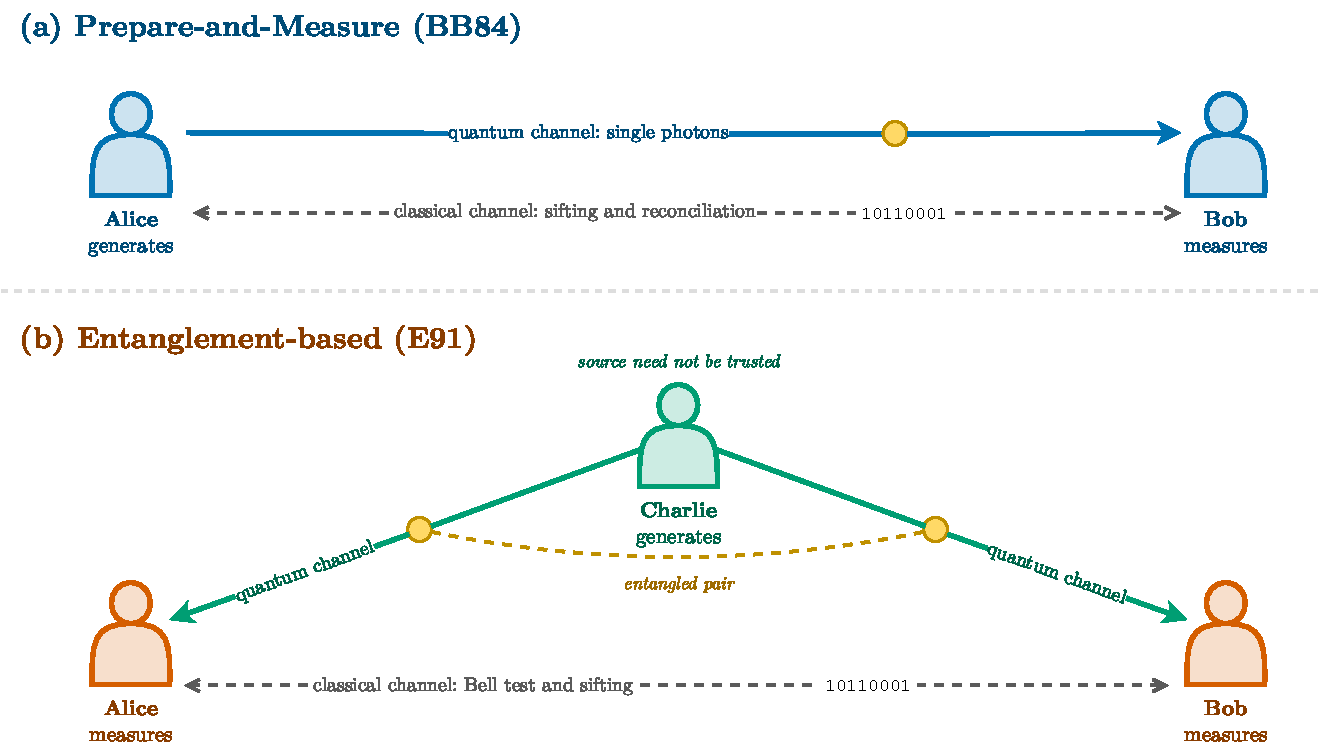
\includegraphics[width=\linewidth]{figures/chapter4/qkd_paradigms.pdf}
  \caption{The two principal QKD paradigms differ in where the photon source
  sits and how much it must be trusted. In \textbf{(a)} prepare-and-measure
  (BB84), Alice hosts a \emph{trusted} source, preparing photons in randomly
  chosen non-orthogonal bases and sending them to Bob over a quantum channel;
  basis sifting and reconciliation proceed over a classical channel. In
  \textbf{(b)} entanglement-based QKD (E91), a central party (Charlie) operates
  a source that \emph{need not be trusted}, distributing one photon of each
  entangled pair to Alice and one to Bob; security is instead certified by a
  Bell-inequality test ($S>2$), so genuine entanglement---rather than trust in
  the source---guarantees secrecy. In both paradigms, Alice and Bob exchange
  basis and reconciliation information over an authenticated classical channel
  and distil a shared secret key (matching bit strings); any eavesdropping on
  the quantum channel raises the quantum bit error rate (QBER) and is thereby
  detectable.}
  \label{fig:qkd-paradigms}
\end{figure}

Entanglement-based schemes are particularly crucial for the vision of a quantum internet~\cite{Wehner2018}. They enable device-independent QKD and supply the entanglement resource on which quantum teleportation and entanglement swapping rely---the primitives that, in the quantum repeaters of Section~\ref{sec:qsrc-distance}, route quantum states across multi-hop topologies rather than over single point-to-point links.

\section{The BB84 Protocol and Raw Key Generation}
\label{sec:qkd-dpu-bb84}

To understand the computational burden of QKD, it is necessary to first examine how raw key material is generated. The prototypical example is the BB84 protocol~\cite{bennett1984quantum}, a prepare-and-measure scheme that serves as the foundation for the synthetic quantum source evaluated in this chapter.

In BB84, Alice seeks to share a secret key with Bob. She generates a sequence of random classical bits and encodes each into a single photon. While nearly every textbook renders BB84 using $\uparrow\!\rightarrow\!\nearrow\!\searrow$ arrows denoting polarization encoding, we take the road less travelled here and carry the bits in the photon's \emph{frequency} (spectral) degree of freedom instead, aligning with the states produced by the quantum sources of Chapter~\ref{ch:quantum-sources}. BB84 is agnostic to the physical carrier: any pair of mutually unbiased bases suffices.

For each bit, Alice randomly chooses one of two such bases. In the frequency basis ($f$) she localizes the photon in one of two discrete frequency bins, encoding a `0` as $|f_0\rangle$ and a `1` as $|f_1\rangle$. In the phase basis ($\phi$) she instead prepares an equal superposition of the two bins, encoding a `0` as $|{+}\rangle$ and a `1` as $|{-}\rangle$, where $|{\pm}\rangle = (|f_0\rangle \pm |f_1\rangle)/\sqrt{2}$ are the two bins combined with relative phase $\varphi=0$ and $\varphi=\pi$, respectively.

Alice transmits this stream of single photons to Bob over a quantum channel, such as a dedicated optical fiber. Upon receiving a photon, Bob must measure its state to recover the bit. However, because he does not know which basis Alice used, he randomly and independently chooses a measurement basis ($f$ or $\phi$) for each incoming photon: the frequency basis is read out by a filter that resolves which bin the photon occupies, while the phase basis requires electro-optically mixing the two bins before detection so that their relative phase becomes measurable.

If Bob guesses the same basis Alice used, quantum mechanics guarantees he will measure the correct bit (in an ideal, noiseless system). If he guesses the wrong basis, his measurement result is completely uncorrelated with Alice's original bit. Furthermore, the no-cloning theorem prevents an eavesdropper, Eve, from copying the photons to measure later. If Eve attempts to intercept and measure the photons in transit, her own random basis choices will inevitably disturb the quantum states, introducing a detectable error rate into the channel.

The quantum transmission concludes with Alice and Bob each holding a string of bits (Bob's measurements and Alice's original bits) and a corresponding array of the bases they used. Table~\ref{tab:bb84-sifting} traces this process over a short sequence of rounds, showing how only the rounds in which their independently chosen bases happen to agree survive into the sifted key. At this point, the quantum physical layer's job is complete. However, this raw key is entirely unusable for cryptography: it is riddled with errors from basis mismatches, optical channel noise, and potential eavesdropping.

\begin{table}[htbp]
  \centering
  \caption{A worked BB84 example over eight transmission rounds, using
  frequency-bin rather than the customary polarization encoding. Alice encodes
  each random bit in a randomly chosen basis---the frequency basis
  ($f$: $|f_0\rangle$ for~0, $|f_1\rangle$ for~1) or the phase basis
  ($\phi$: $|{+}\rangle$ for~0, $|{-}\rangle$ for~1, with
  $|{\pm}\rangle=(|f_0\rangle\pm|f_1\rangle)/\sqrt{2}$)---and Bob measures in his
  own randomly chosen basis. When the bases agree, Bob recovers Alice's bit;
  when they disagree, his outcome is uncorrelated ($-$) and the round is
  discarded during sifting. The surviving bits form the raw sifted key, from
  which errors are still removed by the classical post-processing pipeline of
  Section~\ref{sec:qkd-dpu-bottleneck}.}
  \label{tab:bb84-sifting}
  \begin{tabular}{l*{8}{c}}
    \toprule
    Round & 1 & 2 & 3 & 4 & 5 & 6 & 7 & 8 \\
    \midrule
    Alice's bit          & 0 & 1 & 1 & 0 & 1 & 0 & 0 & 1 \\
    Alice's basis        & $f$ & $\phi$ & $f$ & $\phi$ & $f$ & $\phi$ & $f$ & $\phi$ \\
    State sent           & $|f_0\rangle$ & $|{-}\rangle$ & $|f_1\rangle$ & $|{+}\rangle$ & $|f_1\rangle$ & $|{+}\rangle$ & $|f_0\rangle$ & $|{-}\rangle$ \\
    Bob's basis          & $f$ & $f$ & $f$ & $\phi$ & $\phi$ & $\phi$ & $\phi$ & $\phi$ \\
    Bob's bit            & 0 & $-$ & 1 & 0 & $-$ & 0 & $-$ & 1 \\
    \midrule
    Bases agree?         & \checkmark & $\times$ & \checkmark & \checkmark & $\times$ & \checkmark & $\times$ & \checkmark \\
    Sifted key           & 0 & & 1 & 0 & & 0 & & 1 \\
    \bottomrule
  \end{tabular}
\end{table}

\section{The Computational Bottleneck of Post-Processing}
\label{sec:qkd-dpu-bottleneck}

To transform this error-riddled raw key into a secure, usable cryptographic key, Alice and Bob must execute a classical post-processing pipeline. While the physical generation, transmission, and detection of quantum states (as discussed in Chapter~\ref{ch:quantum-sources}) have seen tremendous advancements, executing this classical pipeline at scale introduces a significant computational load. This pipeline consists of several computation-heavy stages:

\begin{enumerate}
    \item \textbf{Sifting:} Alice and Bob exchange their basis choices over an authenticated classical channel and discard measurements where incompatible bases were used.
    \item \textbf{Error Estimation:} A subset of the sifted bits is publicly compared to estimate the quantum bit error rate (QBER). Because the protocol assumes all errors are caused by an eavesdropper, the QBER bounds the maximum information Eve could have gained.
    \item \textbf{Information Reconciliation:} To resolve discrepancies between Alice's and Bob's strings caused by channel noise, the parties perform forward error correction. This is typically achieved using rate-adaptive Low-Density Parity-Check (LDPC) codes or the Cascade protocol. For LDPC, the receiver executes iterative belief propagation (e.g., the min-sum algorithm) to converge on the correct string.
    \item \textbf{Privacy Amplification:} Once the strings match, Alice and Bob compress them using a universal hash function (such as Toeplitz matrix multiplication) to erase any partial information the eavesdropper might hold, yielding the final, perfectly secret key.
\end{enumerate}

The computational complexity of this pipeline is substantial, particularly during information reconciliation and privacy amplification. As the QBER rises due to optical channel impairments or distance, LDPC decoding requires larger matrices, more iterations, and lower code rates, scaling the computational burden exponentially. Furthermore, all classical communication during these steps must be strictly authenticated to prevent man-in-the-middle attacks.

\section{Programmable Network Hardware and the Trust Boundary}
\label{sec:qkd-dpu-trust}

Datacenter networks operate at terabit-per-second scales, relying heavily on low-latency, high-throughput transport protocols. Traditionally, QKD post-processing has been executed either on rigid FPGA appliances or on general-purpose host CPUs. Both integration models suffer from structural flaws when deployed in high-performance environments.

Dedicating host CPU cycles to cryptographic key distillation becomes economically and operationally prohibitive. Executing iterative LDPC belief propagation and large-scale Toeplitz hashing on x86 processors consumes the compute resources the datacenter is built to provide. Alternatively, offloading these tasks to a standalone FPGA appliance solves the compute bottleneck but fragments the trust boundary: the distilled key must still be securely transported from the appliance to the server's network interface card (NIC) where the actual data encryption takes place. Whether using an external Key Management System (KMS) or transferring the keys across the host's PCIe bus, this handoff adds latency, restricts key-injection throughput, and exposes the plaintext key material to potential software or bus vulnerabilities.

This chapter proposes and evaluates an architecture that collapses the key generation and key consumption trust boundaries into a single network device. By offloading the entire post-processing pipeline to the Arm cores of an NVIDIA BlueField-3 Data Processing Unit (DPU), the architecture isolates the key material from the host CPU. The DPU natively performs sifting, LDPC error correction, and privacy amplification, ensuring the host CPU utilization remains at zero.

\section{Quantum-Secured Datacenter Fabrics (Q-RDMA)}
\label{sec:qkd-dpu-rdma}

The primary motivation for offloading QKD to the DPU is to protect latency-sensitive datacenter workloads without degrading their performance. Modern distributed training clusters, storage backends, and high-frequency trading platforms rely on Remote Direct Memory Access (RDMA) over Converged Ethernet (RoCEv2) to bypass the host kernel and achieve microsecond latencies.

Standard, software-based encryption fundamentally breaks RDMA by forcing traffic back through the host's CPU and memory subsystem. To securely encrypt RDMA, the cryptography must be applied inline by the network hardware.

By executing QKD post-processing entirely within the DPU, the resulting quantum-secure keys never cross the PCIe bus to the host. Instead, they are formatted as Security Associations (SAs) and injected seamlessly into the DPU's local hardware IPsec or MACsec encryption engines. This enables quantum-secured RDMA (Q-RDMA). The data plane encryption operates transparently at line rate, while the continuous distillation of fresh keys occurs asynchronously on the DPU's Arm cores. Consequently, the fabric's latency and throughput remain completely isolated from the heavy computational cost of QKD key generation. To evaluate this architecture under stable, reproducible error conditions---rather than at the mercy of the environmental drift, dark counts, and afterpulsing that plague physical optical hardware---the included paper emulates the qubit transmission layer with a synthetic BB84 source that injects controlled QBER profiles, while running the entire post-processing pipeline, key derivation, and hardware IPsec injection on real BlueField-3 silicon.

\section{Contribution and Articles}
\label{sec:qkd-dpu-context}

This chapter is built around one contribution (P3), the manuscript \enquote{QKD Post-Processing Offload on BlueField-3 DPUs: Towards Quantum-Secured RDMA in Datacenter Fabrics}.

This manuscript was accepted and presented at IEEE Quantum Week (QCE). The paper contributes a complete hardware/software co-design strategy for offloading the classical communication channel, LDPC decoding, and IPsec key injection onto a DPU. This demonstrates that continuous distillation of fresh keys can occur asynchronously on programmable network hardware without burdening the host CPU.

Beyond this article, the work on quantum-secured networking also contributed to several filed patent applications, \enquote{Multi-Hybrid Cryptographic Key Exchange (MHKE)} (I2) and \enquote{ROSE-QKD: Receiver-Only, Semi-Honest Emitter Quantum Key Distribution} (I3), together with a draft application on \enquote{Capability-Based Authentication of Quantum Nodes via Statistical Analysis} (I4). These inventions, which extend the architectural concepts evaluated in this chapter, are reported at title level among the patents in the List of Publications.

This paper addresses the core integration challenge outlined in \textbf{RQ2}: how to make QKD systems scalable and practical in high-performance datacenters. It closes the gap between quantum key generation (explored in Chapter~\ref{ch:quantum-sources}) and deployable datacenter security by offloading the full post-processing pipeline---sifting, error estimation, reconciliation, and privacy amplification---onto a BlueField-3 DPU. By injecting the distilled keys directly into the DPU's hardware encryptors, quantum-secured RDMA retains line-rate latency and throughput.

\includedpaper{P3}{QKD Post-Processing Offload on BlueField-3 DPUs: Towards Quantum-Secured RDMA in Datacenter Fabrics}{meyer2026qkd}{source-materials/papers/camera-ready/QKD_PostProc_DPUs.pdf}

\section{Discussion and Transition}

While QKD offers information-theoretic security for key distribution, it requires specialized optical hardware and dedicated fiber links, making it challenging to deploy ubiquitously across all network segments. To achieve comprehensive quantum-safe security, QKD must be complemented by PQC---classical cryptographic algorithms believed to be secure against quantum computers. The next chapter explores this complementary approach, shifting the focus from quantum-generated security material to the execution of PQC algorithms on the same programmable network infrastructure used here for QKD post-processing.


\part{Post-Quantum Cryptography}
\label{part:pqc}

\chapter{DPU-Accelerated Post-Quantum Cryptography}
\label{ch:dpu-pqc}

\section{Post-Quantum Cryptography and Its Deployment Cost}
\label{sec:pqc-background}

Post-quantum cryptography (PQC) represents the computationally secure counterpart to QKD.
It replaces the integer factorization and discrete logarithm problems vulnerable to Shor's
algorithm with entirely different mathematical structures believed to resist both classical
and quantum cryptanalysis. The transition focuses on two main primitive types: key
encapsulation mechanisms (KEMs), which establish a shared symmetric key over an insecure
channel, and digital signatures, which provide authentication and non-repudiation.

\subsection{Algorithmic Families and Characteristics}

The standardized and candidate algorithms studied in this part vary drastically in their
underlying mathematics, leading to profound differences in computational structure,
memory footprint, and message sizes~\cite{nistfips203,nistfips204,nistfips205,nistir8545}.

\begin{itemize}
    \item \textbf{Lattice-Based Cryptography:} Algorithms like ML-KEM (formerly Kyber) and
    ML-DSA (formerly Dilithium) rely on the hardness of the module learning with errors (MLWE)
    problem. They offer an excellent balance: fast execution times, moderate key and ciphertext
    sizes, and efficient hardware implementations. However, their reliance on polynomial sampling
    and rejection sampling introduces variable timing that must be carefully managed to avoid
    side-channel leaks.
    \item \textbf{Code-Based Cryptography:} Algorithms like HQC (Hamming Quasi-Cyclic) rely on
    the hardness of decoding random linear codes. While their encryption and decryption operations
    are fast, they suffer from significantly larger public keys and ciphertexts compared to lattices.
    Additionally, their operations involve large, dense bit-vector multiplications that have distinct
    memory access patterns~\cite{meyer2026hqc}.
\end{itemize}

Table~\ref{tab:pqc-comparison} summarizes these structural differences.

\begin{table}[htbp]
\centering
\caption{Comparison of selected Post-Quantum Cryptographic primitives and their deployment profiles. Sizes and operations are approximations based on NIST security category 3~\cite{nistfips203,nistfips204,nistir8545}.}
\label{tab:pqc-comparison}
\renewcommand{\arraystretch}{1.3}
\footnotesize
\begin{tabularx}{\textwidth}{llcrr>{\raggedright\arraybackslash}X}
\toprule
\textbf{Algorithm} & \textbf{Family} & \textbf{Type} & \textbf{PK (B)} & \textbf{CT/Sig (B)} & \textbf{Compute profile} \\
\midrule
ML-KEM-768 & Lattice & KEM & 1,184 & 1,088 & Fast polynomial arithmetic; SIMD-friendly (AVX/Neon). \\
ML-DSA-65 & Lattice & Signature & 1,952 & 3,309 & Rejection sampling; highly variable timing. \\
HQC-192 & Code & KEM & 4,522 & 9,026 & Bitwise math; memory-bound (large keys). \\
\bottomrule
\end{tabularx}
\end{table}

\subsection{Deployment and Architectural Constraints}

For networked systems, the migration to PQC is not finished when a NIST standard is published.
A mechanism that executes efficiently in a single-threaded benchmark may behave disastrously
under datacenter provisioning constraints.

Integrating PQC into protocols like TLS 1.3 or IPsec requires transmitting much larger
public keys and ciphertexts during handshakes. This can trigger IP fragmentation, increasing
latency and packet-loss probability. Furthermore, datacenters handle thousands of connections
per second. KEM decapsulation and signature verification must therefore be deeply batched.
Lattice schemes, with their variable-time rejection sampling, batch poorly on SIMD architectures
because a single long-running sample stalls the entire vector lane.

Consequently, the central questions are architectural: where should the cryptographic work run,
how should requests be batched, how much latency can the service mesh tolerate, and which
memory buses become bottlenecks? These are the questions that motivate offloading PQC onto
the DPU substrate introduced in Chapter~\ref{ch:background}, and they organize the two
contributions that follow.

\section{Contribution and Articles}

This chapter is built around two contributions that study how post-quantum cryptographic workloads can be executed efficiently on heterogeneous, programmable network hardware.

The first contribution (P4), \enquote{Offloading Post-Quantum Cryptography to Data Processing Units: A Performance Analysis of HQC Key Encapsulation}, analyzes the offload of HQC key encapsulation to a BlueField DPU and characterizes the resulting performance.
% TODO: Record the author's specific contributions and co-author context for P4.

The second contribution (P5), \enquote{GPU-Accelerated Post-Quantum Cryptography on Embedded DPU Architecture}, develops and evaluates a heterogeneous DPU architecture that places GPU compute directly in the network datapath to accelerate post-quantum cryptography across CPU, GPU, and DPU resources.
% TODO: Record the author's specific contributions and co-author context for P5.

Beyond these articles, the work on post-quantum cryptographic offload also contributed to a filed patent application, \enquote{Computational Offloading of Operations Necessary for Post-Quantum Cryptography on Network Interface Cards}, reported at title level among the patents in the List of Publications (page~\pageref{listPublications}).

TODO: Synthesize the findings across HQC offload and heterogeneous DPU acceleration, including what they reveal about bottlenecks, host interaction, and deployment constraints, and transition from isolated cryptographic acceleration to full application pipelines that combine data movement, AI workloads, and PQC.

\includedpaper{P4}{Offloading Post-Quantum Cryptography to Data Processing Units: A Performance Analysis of HQC Key Encapsulation}{meyer2026hqc}{source-materials/papers/camera-ready/hqc-pqc-offload-bluefield-dpu-ieee-access-2026-published.pdf}

\includedpaperpending{P5}{GPU-Accelerated Post-Quantum Cryptography on Embedded DPU Architecture}{meyer2026heterogeneous}

\chapter{End-to-End Post-Quantum Security for AI Pipelines}
\label{ch:ai-pipelines}

% Allow a tall figure to occupy the bottom of a text page (default
% \bottomfraction of 0.3 is too small for the panoptic-segmentation figure).
\renewcommand{\bottomfraction}{0.55}
\renewcommand{\textfraction}{0.1}

Chapter~\ref{ch:dpu-pqc} demonstrated that post-quantum cryptographic primitives can be accelerated efficiently on programmable network hardware. However, evaluating an algorithm in isolation, where a key encapsulation mechanism or a digital signature is the only workload on the processor, provides an incomplete picture of datacenter deployment. In production, cryptography is never an isolated benchmark. It is merely one stage in a continuous, contention-prone data path, forced to share processors, memory bandwidth, and trust boundaries with the very application it protects.

To evaluate post-quantum security realistically, one must therefore evaluate it within a live pipeline. This chapter carries the post-quantum primitives into an end-to-end AI workload. It focuses on the ingest-and-inference path, where cryptography must execute alongside decoding, preprocessing, and the execution of the model itself. The central problem shifts from algorithmic speed to architectural placement: where should the secure channel be terminated so that the cryptography does not steal capacity from the revenue-generating application accelerator?

\section{The AI Pipeline}
\label{sec:ai-pipeline}

An AI pipeline is a continuous lifecycle rather than a single computational step. It begins with data ingestion, where raw signals, such as high-resolution video frames, audio streams, or sensor telemetry, are collected at the edge and transmitted to the datacenter. Before this raw data can be fed into a neural network, it must be decoded, normalized, and preprocessed into an application-ready tensor format.

\begin{figure}[htbp]
  \centering
  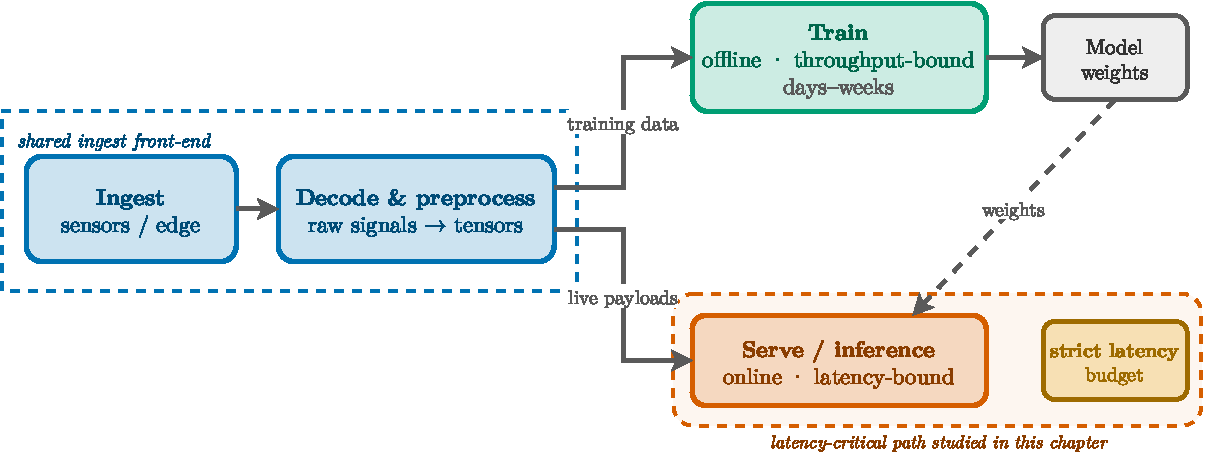
\includegraphics[width=\linewidth]{figures/chapter6/pipeline_anatomy.pdf}
  \caption{The end-to-end data lifecycle in an AI pipeline. Data is ingested from the edge and preprocessed into tensors, which then drive offline training and online, real-time inference. While training optimizes model weights for throughput, inference applies those weights to live payloads under strict latency budgets.}
  \label{fig:pipeline-anatomy}
\end{figure}

Once data is ingested and shaped, it drives two distinct phases: training and inference. Training is typically a throughput-oriented, offline process where massive datasets are consumed to optimize model weights over days or weeks. Inference, by contrast, is a latency-critical, online process. In a real-time system, the entire ingest-to-inference path must complete within a strict temporal budget. For example, a system processing live video might need to ingest, decode, preprocess, and execute inference within a hard per-frame deadline.

To meet these budgets, the pipeline distributes work across heterogeneous hardware. General-purpose host CPUs traditionally handle network I/O and orchestration. Dedicated application accelerators, primarily GPUs, execute the dense matrix multiplications required for model training and inference. More recently, DPUs have been introduced to offload network packet processing and infrastructure tasks. The performance of the pipeline depends entirely on how effectively work is routed among these components to avoid stalls and contention.

\section{The Economics of Secure Inference}
\label{sec:end-to-end-economics}

Serving a modern artificial intelligence model is fundamentally an exercise in resource accounting. Inference now dominates the economics of AI, accounting for 60\% to 90\% of total machine learning compute demand at major cloud providers~\cite{luccioni2024power, xing2026ai}. This share is expected to grow as static, single-pass inference gives way to dynamic reasoning and agentic workflows, where test-time scaling spends far more compute per query~\cite{kim2026cost}. The application accelerator---typically a GPU---is the scarce and expensive resource in the datacenter. Its economic value reduces to a single metric: the fraction of its cycles spent on revenue-generating model execution. Every cycle the accelerator spends on infrastructure or security tasks is a cycle it does not spend serving requests.

Adding mandatory post-quantum cryptography to this pipeline introduces a strict penalty. Every incoming payload must be authenticated and decrypted (e.g., via AES-GCM, keyed by an ML-KEM session), and this work consumes a fixed amount of time and compute. On the most resource-constrained ingestion endpoints, this symmetric stage may instead be carried by a lightweight authenticated cipher such as the NIST-selected ASCON, which targets exactly such power- and memory-limited devices~\cite{cagua2025ascon}. This penalty manifests simultaneously as a latency threat and a throughput tax.

\begin{figure}[b]
  \centering
  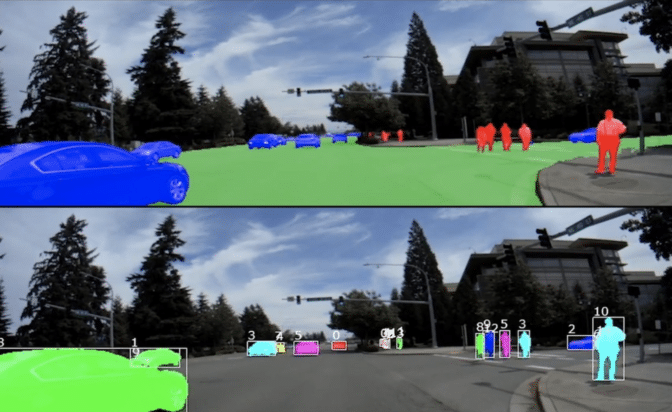
\includegraphics[width=0.6\linewidth]{figures/chapter6/panoptic_segmentation.png}
  \caption{Real-time in-car panoptic perception on an embedded NVIDIA Jetson AGX platform. The top panel labels object categories (e.g., cars blue, pedestrians red, drivable space green); the bottom panel separates individual instances with per-object bounding boxes and IDs~\cite{cvijetic2019panoptic}.}
  \label{fig:panoptic-segmentation}
\end{figure}

On the latency side, a modern perception pipeline might have just tens of milliseconds to carry a frame from the wire to a fully parsed scene, such as the dense object detection and decision making required for autonomous vehicles (Figure~\ref{fig:panoptic-segmentation}). Because decoding and preprocessing already consume a significant portion of that budget~\cite{kang2020preprocessing}, adding milliseconds of cryptographic work threatens the hard per-frame deadline. On the throughput side, any accelerator capacity spent on decryption is capacity subtracted from serving. This lowers the sustainable batch size and the number of concurrent requests. Crucially, this tax is paid on every frame, on every node, for the life of the deployment.

Because the threat model leaves no room to opt out of authentication and decryption, the computational cost of security cannot be eliminated. It can only be relocated. When security tasks cannibalize the accelerator, their true cost is measured in displaced inference.

\section{The Termination Boundary}
\label{sec:end-to-end-termination}

If the cost of security is best managed by relocating it, the next logical question is where it should be placed. A critical design choice for any secure pipeline is therefore determining its termination boundary: the exact point where the secure channel ends, the payload is decrypted, and application processing begins.

The conventional placements for terminating this pipeline are both unsatisfactory. Performing authentication and decryption on the host CPU consumes general-purpose cycles and, more importantly, leaves decrypted payloads and key material resident in the host's memory. This places them inside the host trust domain, where a compromised operating system or hypervisor can observe them. Alternatively, offloading the cryptographic and preprocessing work to the application accelerator (the GPU) resolves the CPU bottleneck but triggers the exact economic failure described above: it steals capacity from the primary workload that the accelerator was provisioned to run. Neither option preserves the latency budget while keeping plaintext out of the host trust domain.

The architecture evaluated in this chapter resolves this placement dilemma by terminating the secure channel at network ingress on the DPU, before payloads ever reach the host. As each payload arrives, the DPU's general-purpose Arm cores authenticate it, decrypt it, and perform the necessary decoding and preprocessing. Only the application-ready data is then transferred across the PCIe bus to the host or accelerator. Figure~\ref{fig:end-to-end-pipeline} contrasts this DPU-terminated path with the conventional host- and accelerator-centric paths.

\begin{figure}[t]
  \centering
  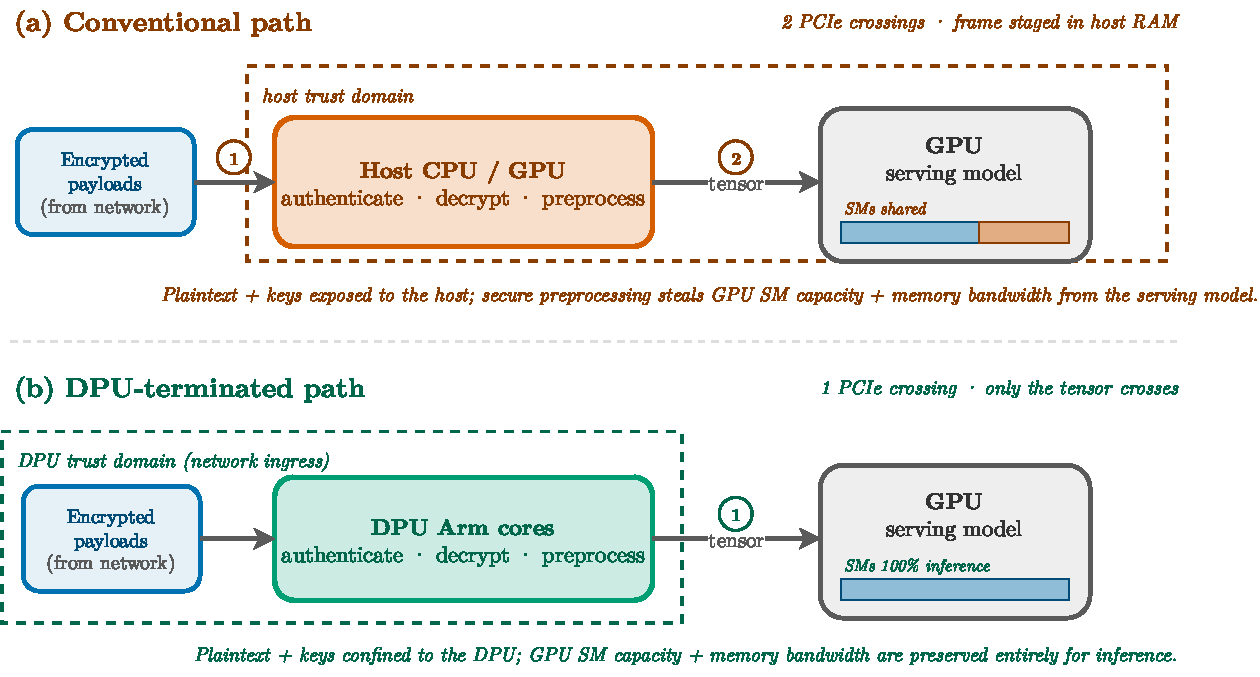
\includegraphics[width=\linewidth]{figures/chapter6/ai_pipeline.pdf}
  \caption{Two placements for the secure preprocessing of a real-time inference
  feed. In the \textbf{conventional path} (top), the host, or an offloaded GPU,
  authenticates, decrypts, and preprocesses each payload. In the
  \textbf{DPU-terminated path} (bottom), the DPU's Arm cores do this work at
  network ingress, so only application-ready data crosses into the GPU.}
  \label{fig:end-to-end-pipeline}
\end{figure}

This placement delivers two benefits at once. It preserves the application accelerator's capacity for the primary workload, since the decode, decrypt, and preprocess stages no longer compete for it. It also confines plaintext data and key material to the DPU, isolating them from the host trust domain and shrinking the attack surface to the network device itself. The design thus turns the DPU from a mere offload target into a security boundary. This is the same architectural move made for QKD key material in Chapter~\ref{ch:qkd-dpu}, now applied to an application data plane.

\section{Contribution and Articles}
\label{sec:end-to-end-context}

To evaluate this architectural placement, this chapter uses real-time image inference as a concrete testbed. Real-time inference represents a specific, demanding case of the ingest-and-inference path. The evaluation is built around one contribution (P6), \enquote{Real-Time Post-Quantum Secured Image Pipeline on NVIDIA BlueField-3 DPU}, which realizes and evaluates the DPU-terminated architecture on real hardware. This addresses \textbf{RQ1} at the level of a complete application pipeline.

This manuscript is under review at the IEEE International Conference on Algorithms and Architectures for Parallel Processing (ICA3PP). The paper implements a real-time, post-quantum-secured image pipeline on an NVIDIA BlueField-3 DPU. It offloads both image I/O and the cryptographic stages (ML-KEM key establishment and ML-DSA authentication bootstrapping a symmetric per-frame data plane) from the host onto the DPU's Arm cores, ultimately delivering an inference-ready tensor to the GPU. 

In this testbed, the pipeline runs against a hard per-frame budget. The headline results establish that the approach is not merely secure but real-time. On a single Arm core, the secure receive path sustains 1080p video at 85~frames per second for JPEG and 98~frames per second for TIFF. The per-frame post-quantum stage consumes only 23\% of the 30~fps budget for a raw 1080p payload. Post-quantum protection, in other words, fits comfortably within a real-time image-inference pipeline when the work is placed on the DPU.

Read against Chapter~\ref{ch:dpu-pqc}, this contribution completes Part~\ref{part:pqc}'s argument. The isolated-primitive studies showed that post-quantum cryptography can be offloaded efficiently. The pipeline study shows that the offload advantage (specifically preserving accelerator capacity, keeping the host trust domain clear, and meeting strict deadlines) survives contact with a full, contention-prone application workload.

% EDGE AI is a Springer LNCS single-column PDF with very wide side margins
% (~130pt each). Trimming them (left bottom right top, in pt) keeps the text
% from being shrunk too far by the book-page rescaling; values leave ~24pt of
% clearance inside the tightest measured ink margin so nothing is clipped.
\includedpaper[trim=110 103 103 56, clip]{P6}{Real-Time Post-Quantum Secured Image Pipeline on NVIDIA BlueField-3 DPU}{meyer2026edgeai}{source-materials/papers/camera-ready/EDGEAI.pdf}

\section{Part II Epilogue}
\label{sec:end-to-end-discussion}

The transition to post-quantum cryptography is often framed as a purely mathematical challenge, but as Part~\ref{part:pqc} has demonstrated, the true challenge is architectural. The heavy computational requirements of these new primitives threaten to overwhelm the host processors and application accelerators that power the modern datacenter. Addressing this requires moving cryptography out of the host and into the network infrastructure. By leveraging DPUs to isolate and accelerate this burden---whether by offloading memory-bound schemes to Arm cores, batching lattice schemes on embedded GPUs, or terminating an entire secure AI pipeline at network ingress---the central claim holds: post-quantum protection can be made practical at scale by treating security and the network device as a single co-designed data path. The DPU is no longer just a network interface; it becomes the boundary where the secure channel ends and the application begins.

This conclusion marks a pivotal shift in the scale of the thesis. Thus far, the analysis has followed a progressive zoom outward. Part~\ref{part:qkd} focused on the device level, examining foundational quantum security mechanisms. Part~\ref{part:pqc} zoomed out to the node level, evaluating how cryptographic algorithms and pipelines can be accelerated on DPUs without crippling application performance. 

Part~\ref{part:infra} now completes this zoom by expanding the focus to the entire datacenter and reframing it as a security problem in its own right. It examines the fabric wiring everything together and the multi-tenant confidential cluster operating as a live system. As the scale expands, the driving question changes: does the system survive adversarial operation? Parts I and II of this thesis treated the DPU and the optical fabric beneath it as a cooperative, trustworthy substrate. Part III stops trusting that substrate. Rather than focusing on the device physics of individual components, it interrogates the systemic and structural behaviours of the hardware, first turning them into an attack surface and then reclaiming them as the defender's vantage point. By examining how lower-layer routing, timing, and power characteristics can undermine higher-layer security assumptions---and how the same signals can be turned back into a means of defending them---Part III directly addresses RQ4.

% Restore default float placement fractions for subsequent chapters.
\renewcommand{\bottomfraction}{0.3}
\renewcommand{\textfraction}{0.2}


\part{Programmable Datacenter Infrastructure}
\label{part:infra}

\chapter{Infrastructure Attacks}
\label{ch:rdma}

Security proofs reason about an idealized machine: one that computes in constant time, emits nothing an observer can measure, and moves bytes over a channel that reveals only their ciphertext. Real deployments run on a physical substrate that violates every one of those assumptions. Transistors consume power as they switch, processors take data-dependent time, and packets traverse a shared fabric whose routing and timing are visible to anyone positioned to watch. Where the preceding parts trusted this substrate to faithfully carry the quantum and post-quantum mechanisms built on top of it, Part~\ref{part:infra} makes the substrate itself the object of study, at the scale of the whole datacenter. This chapter opens that shift on the offensive: it treats the substrate not as a neutral medium but as an attack surface, escalating from the device-level behaviour of individual chips to the datacenter-scale behaviour of the fabric that connects them.

\section{Hardware and Node-Level Infrastructure}
\label{sec:node-infra}

The lowest layer of the physical substrate---the individual silicon chips and local hardware components---presents the most fundamental attack surface. At this node level, the physical and structural behaviour of the hardware exposes secret state directly to co-located or physically proximate adversaries.

\subsection{Passive Side Channels}
\label{sec:passive-side-channels}

Early demonstrations of physical vulnerability focused on \emph{side channels}, a framing that carries an implicit assumption: that the adversary is a passive observer who reads whatever the substrate happens to leak. In the context of infrastructure attacks, classic side channels are a passive, single-chip special case.

The Advanced Encryption Standard (AES) provides a well-known demonstration. While mathematically unbroken, early implementations were famously defeated by differential power analysis (DPA)~\cite{kocher1999differential}. DPA exploits the fact that the power consumed by a processor depends on the data it is processing. By measuring the power drawn while the device encrypts many known plaintexts, an attacker can statistically correlate the physical traces with hypotheses about the secret key. The correct guess produces a pronounced statistical spike, while incorrect ones vanish into noise.

This allows an attacker to recover the secret key one byte at a time. Instead of an exhaustive search that grows exponentially with the key length, the attack breaks the problem into independent, byte-sized guesses. As illustrated in Figure~\ref{fig:dpa}, an unprotected AES-128 implementation on a commodity microcontroller yields its complete 16-byte key through a sequence of trivial single-byte attacks~\cite{lo2016power}. The mathematics is untouched; the physical implementation simply hands the key over.

% Figs reprinted from Lo et al. (2016) under Taylor & Francis thesis-use permission
% (single excerpt, up to 3 figures/tables). Required acknowledgement is in the caption.
\begin{figure}[htbp]
  \centering
  \begin{subfigure}{0.49\linewidth}
    \centering
    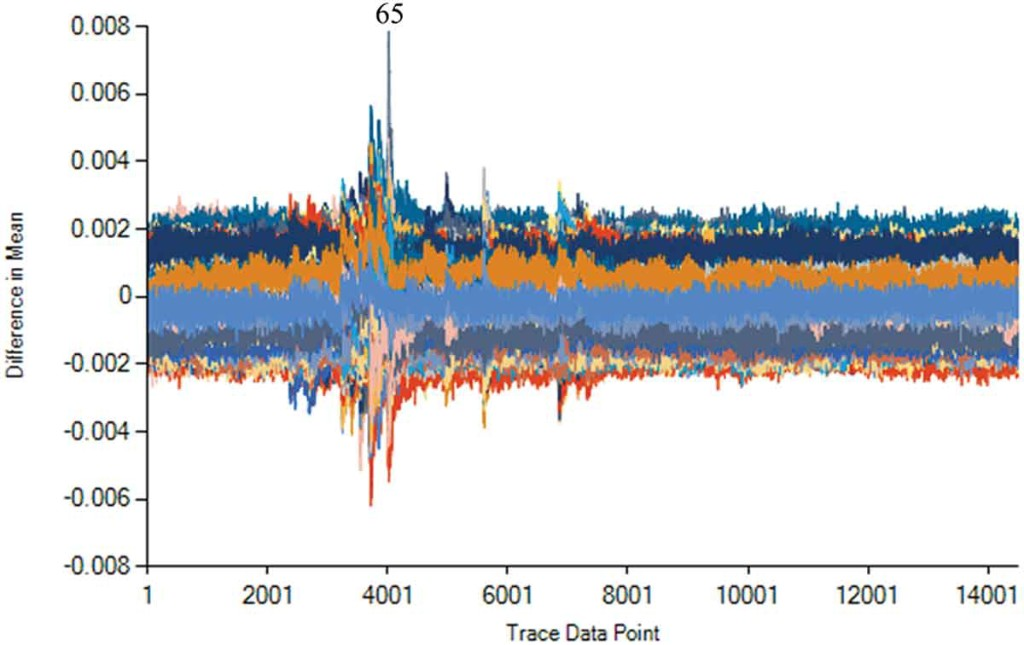
\includegraphics[width=\linewidth]{figures/chapter7/dpa_1byte.png}
    \caption{Recovering a single key byte.}
    \label{fig:dpa-1byte}
  \end{subfigure}
  \hfill
  \begin{subfigure}{0.49\linewidth}
    \centering
    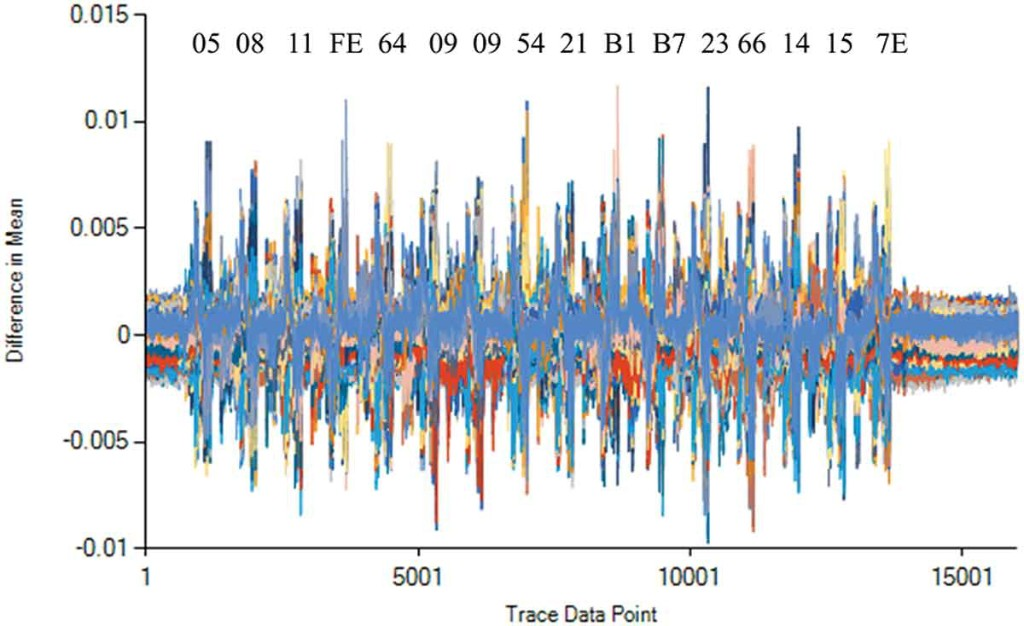
\includegraphics[width=\linewidth]{figures/chapter7/dpa_16byte.png}
    \caption{Recovering the full 16-byte key.}
    \label{fig:dpa-16byte}
  \end{subfigure}
  \caption{Differential power analysis against an unprotected AES-128 S-box, using a difference-of-means power model over traces captured from a commodity microcontroller. \textbf{(a)}~For a single key byte, the correct candidate (labelled) rises as a pronounced spike above the noise formed by the 255 incorrect guesses. \textbf{(b)}~Attacking each byte position independently recovers the complete 16-byte key without requiring an exponential exhaustive search. Reprinted from O.~Lo, W.~J.~Buchanan, and D.~Carson, ``Power analysis attacks on the AES-128 S-box using differential power analysis (DPA) and correlation power analysis (CPA),'' \emph{Journal of Cyber Security Technology}, \textcopyright~2016, by permission of Informa UK Limited, trading as Taylor \& Francis Group, \url{https://www.tandfonline.com}~\cite{lo2016power}.}
  \label{fig:dpa}
\end{figure}

DPA is one point on a broad spectrum of physical leakage. The same data-dependence surfaces as electromagnetic and acoustic emanation, as data-dependent execution time in code that is not constant-time, and as microarchitectural leakage through shared caches and branch predictors. Quantum protocols expose the same implementation lesson. As discussed in Chapter~\ref{ch:background}, the mathematical security of QKD can be bypassed when the receiver's physical detector behaviour leaks or is driven outside the model assumed by the proof~\cite{lydersen2010hacking}. QKD side-channel attacks are therefore an important and active area of research (TODO: citations).

What unites these examples is that each converts an internal secret, state, or protocol assumption into an externally observable physical quantity that the security proof never modelled. Countermeasures narrow these channels but rarely close them. Masking, hiding, constant-time coding, detector monitoring, and calibration manage the leak but do not eliminate the fact that the proof ultimately runs on hardware.

\subsection{Active Hardware Perturbation}
\label{sec:active-hardware-perturbation}

While passive side channels rely on observing natural emissions, active infrastructure attacks deliberately change the hardware environment. The adversary is no longer limited to what the system reveals during normal operation. They can inject faults, create contention, and then observe whether the protected computation slows down, fails, retries, or produces a distinguishable response.

At the device level, this includes fault injection through voltage or clock glitches, thermal stress, electromagnetic disturbance, or laser and optical probing in systems where the package is physically accessible (TODO: citation). A carefully timed clock or voltage glitch can violate the processor's normal timing assumptions and cause an instruction, branch, or authentication check to be skipped, turning a physical disturbance into a logical bypass. In shared compute systems, the same idea appears as resource manipulation. An attacker co-located on the same physical host might intentionally thrash the shared L3 cache to evict a victim's cache lines, pressure memory bandwidth, or trigger page-placement effects that make the victim's execution more distinguishable. The leak is not simply discovered; it is shaped.

This matters because active perturbation turns infrastructure into a control surface. The attacker can test hypotheses by applying pressure and watching the response. A cryptographic operation may be constant-time in source code, but it still executes on hardware with caches, queues, voltage regulators, thermal limits, and retry mechanisms. Those mechanisms create handles that an adversary can pull.

The same pattern scales beyond a single node. In a larger system, the object being perturbed is not only a cache set or a voltage rail. It can be a shared PCIe path, a storage backend, a scheduler, or the network fabric itself. That shift is what makes infrastructure attacks more than classical side-channel attacks: the manipulated substrate becomes distributed.

\section{Datacenter-Scale Vulnerabilities}
\label{sec:datacenter-scale}

The threat model fundamentally shifts when moving from isolated hardware to multi-tenant, datacenter-scale environments. Both the difficulty and the consequences increase. The adversary may not share a processor socket with the victim, but they can still share switches, uplinks, optical paths, storage systems, congestion domains, and scheduling infrastructure. At the same time, the assets are larger: artificial intelligence (AI) model weights represent millions of dollars in compute time and proprietary intellectual property, while even short disruptions can waste scarce accelerator capacity.

The result is a wider infrastructure attack surface than a single local side channel. A datacenter adversary can learn from passive traffic metadata, including packet timing, burst structure, flow fan-out, and synchronization cadence. They can interfere with availability by creating congestion, inducing retries, or causing stragglers in distributed jobs. They can exploit placement and co-tenancy effects when the scheduler places unrelated workloads on shared resources. They can also target the control plane, where routing, telemetry, orchestration, and accelerator allocation decisions shape what the workload actually experiences.

The common feature is that the security boundary sits above infrastructure that remains shared and measurable. Encryption can hide payloads, but it does not hide when a job communicates, how many peers it talks to, how synchronized its phases are, or how it reacts when the fabric is stressed. At datacenter scale, this metadata is not incidental; it is often enough to reveal workload structure.

\subsection{Congestion and Byzantine Behaviour}
\label{sec:congestion-byzantine}

In a federated learning or multi-tenant cluster, Byzantine workers are nodes that behave like the faulty or treacherous participants in the Byzantine Generals problem: they may follow the protocol sometimes, lie at other times, and coordinate their deviations to confuse the rest of the system. A malicious worker can participate just enough to appear legitimate while sending poisoned gradients, stale updates, or malformed data into the training process. It can also shape its traffic to interfere with the rest of the job by sending at awkward times, bursting into specific collective phases, delaying selected updates, or targeting paths that are likely to be shared with the victim's gradient exchange.

The immediate consequence is availability loss. Distributed training relies on synchronization barriers: the slowest participant in an all-reduce or all-to-all exchange determines when the next iteration can begin. Congestion and selective delay therefore amplify small local disturbances into job-level slowdowns. Even if no secret is extracted, delaying training or inference causes financial damage, degrades service quality, and wastes scarce accelerator time.

The deeper consequence is that perturbation becomes a probe. At the network level, flooding specific switch ports can force the fabric's load balancers to reroute traffic, causing timing skew, queue buildup, and packet reordering. A Byzantine participant can do something similar from inside the workload by changing when and how it communicates. By watching how the victim's traffic cadence changes under controlled contention, the adversary can infer which flows share paths, which phases of the workload are communication-heavy, and where synchronization boundaries occur. The adversary no longer needs to be co-located on the same host; they simply need to share enough infrastructure for their pressure to be visible.

\subsection{The Optical Fabric as an Attack Surface}
\label{sec:fabric-attack-surface}

The optical fabric is the shared physical substrate of the modern accelerator cluster. Its purpose is to make thousands of GPUs, DPUs, storage devices, and hosts behave as if they were connected by a fast, uniform backplane. In practice, that illusion is built from many optical links, switches, queues, and load-balancing decisions. Those mechanisms are normally treated as performance details, but they also determine which paths packets take, when they arrive, and how traffic changes under load.

RDMA is where this fabric behaviour becomes visible to applications. It has become the standard for high-performance datacenter networking because it reaches microsecond latency and line-rate throughput by bypassing the host operating system network stack. Applications communicate directly with network interface card hardware through queue pairs (QPs), typically deployed as RDMA over Converged Ethernet (RoCEv2) over high-throughput optical fabrics.

RDMA's performance comes from removing software from the critical path, but that also moves correctness assumptions closer to hardware. Although RDMA guarantees strict ordering \emph{within} a single QP, its ordering guarantees \emph{across} QPs are weak and depend heavily on fabric load-balancing and optical-switch behaviour. Applications, and the security arguments layered on top of them, nonetheless frequently assume strict cross-QP ordering, a guarantee the specification never promised~\cite{rfc5040, ibta_rocev2}. This is precisely the kind of silent cross-layer assumption that infrastructure attacks exploit.

Modern fabrics expose this weak guarantee through adaptive routing, packet spraying, and multipath forwarding designed to maximize throughput and avoid congested links. These mechanisms are valuable for performance, but they turn the weak cross-QP ordering guarantee into observable reordering and timing skew at the receiver. An adversary who can observe or influence the optical layer, whether through a tapped fibre, a compromised switch, or by deliberately inducing contention from a Byzantine node, obtains a structural channel that both leaks application state and can be actively steered. By flooding specific paths, the attacker forces the fabric's load balancers to reroute the victim's traffic, deterministically altering the arrival order of packets across different QPs.

This structural leakage is particularly damaging for distributed AI training, whose communication is highly regular. Training workloads rely on structured collectives, such as ring or tree all-reduce and all-to-all exchanges, executed at a fixed iteration cadence to synchronize gradients across thousands of GPUs. These patterns are strongly fingerprintable through timing and ordering even when every payload is encrypted. Moving cryptography off the host and onto the fabric does not remove this exposure; it relocates it to a layer where, once structural, it can no longer be patched in software. The adversary does not need to break the encryption protecting the AI weights; they simply need to observe or perturb the fabric to infer the model's architecture, the training progress, or the communication graph.

\section{Contribution and Articles}
\label{sec:rdma-context}

The following article, \textit{Exploiting Cross-QP Ordering in RDMA over Optical Fabrics}, was accepted and presented as an invited paper at the International Conference on Transparent Optical Networks (ICTON) 2026.

This paper grounds the infrastructure-attack argument in a concrete exploit, showing that physical-layer routing behaviour can undermine higher-layer security guarantees. It addresses RQ4 by demonstrating how weak cross-QP ordering and timing behaviour in RDMA over optical fabrics can be turned into an observable channel. By revealing that an adversary can infer application-level state from fabric-level reordering, the paper exposes the limits of purely cryptographic security arguments and motivates the cross-layer analysis that the rest of Part~\ref{part:infra} develops.

\includedpaper{P7}{Exploiting Cross-QP Ordering in RDMA over Optical Fabrics}{meyer2026rdma}{source-materials/papers/camera-ready/cross-qp-ordering-rdma-optical-fabrics-camera-ready.pdf}

\chapter{Infrastructure Defence}
\label{ch:confidential-ai}

The previous chapter treated the infrastructure as an attack surface, reading fabric structure to compromise a system. This chapter inverts that stance. It asks whether the same structural signal that betrays a system to an attacker can be harnessed to defend it, turning the infrastructure from an attack surface into a sensor.

The setting that forces this question is confidential computing. As artificial intelligence models become astronomically expensive to train, protecting model weights and training data is a critical operational requirement. In response, confidential computing encrypts everything the infrastructure operator can see. This creates a profound challenge: once payloads are entirely opaque, what observable signal survives, and can a defender still detect threats using it?

\section{The Defender's Dilemma}
\label{sec:conf-dilemma}

Confidential computing relies on hardware trusted execution environments (TEEs), such as AMD SEV-SNP and Intel TDX, alongside increasingly confidential GPUs featuring encrypted memory, PCIe, and network links (TODO: citation). This architecture protects the tenant workload from both a privileged hypervisor and a malicious infrastructure operator.

However, this introduces a sharp tension: the same cryptographic boundary that shields the tenant also blinds the defender. The infrastructure operator remains responsible for the security and health of the cluster, yet is cryptographically forbidden from inspecting the workloads running on it. Consequently, classical intrusion detection systems (IDS) built on deep packet inspection (DPI) and payload signature matching are rendered entirely useless. While prevention mechanisms are robust, they are not enough; the open problem in confidential AI infrastructure is detection under opacity.

\section{The Datacenter as an Observable System}
\label{sec:conf-observable}

At datacenter scale, the operator is responsible for thousands of confidential jobs that it cannot look inside. The only approach that scales is reading aggregate structure---the datacenter's vital signs---rather than any individual packet's content. Because the operator cannot biopsy the workload, they must read the whole body's telemetry.

In this architecture, the data processing unit (DPU) serves as a privileged vantage point and sensor at every node. It sits below the tenant trust line but remains on the infrastructure side, allowing it to watch metadata without breaking confidentiality. The union of these per-node DPU vantage points turns an otherwise opaque cluster into an observable system. This reframes the DPU into a detection vantage point, extending the focus toward detection and response.

\section{What Signal Survives Encryption}
\label{sec:conf-observability-surface}

To build an observability taxonomy, one must enumerate the surface that survives both encryption and TEE boundaries. This surviving signal includes network metadata (such as packet sizes, timing, inter-arrival rates, flow volumes, and fan-in/fan-out ratios), communication structure (specifically the collective-operation patterns inherent in training), DPU hardware telemetry (including queue depths, DMA and PCIe activity, and hardware counters), and control-plane or attestation events.

AI training makes this observability tractable. AI training traffic is highly regular, characterized by predictable collectives and a fixed iteration cadence. Any deviation from the expected all-reduce rhythm serves as a strong anomaly signal. Consequently, several threats remain detectable without payload access. Data exfiltration, malware beaconing and command-and-control communication, lateral movement, cryptomining, and hijacked or poisoned jobs each perturb the traffic structure, even under encryption.

Because no single layer is legible anymore, the defender must fuse signals across the optical, transport, and DPU-hardware layers. In this context, cross-layer analysis ceases to be a slogan and becomes a literal, necessary method for detection.

\section{Contribution and Articles}
\label{sec:conf-context}

The following articles form the core of this chapter. \textit{Cross-Layer Observability for Intrusion Detection in Confidential AI Training Clusters} was accepted and presented as an invited paper at the International Conference on Transparent Optical Networks (ICTON) 2026. \textit{Obscured, But Not Blind: Systematizing Observability in Confidential AI Training Clusters} is currently under review for journal publication (TODO: confirm venue/status).

These papers contribute to the thesis by charting an arc from exploration to systematization. The first paper explores the design space and trade-offs of AI-based intrusion detection in confidential systems. The second paper systematizes the observable surface that survives encryption and TEE boundaries, validating it with worked-example measurements when payload access is unavailable. Both papers address RQ4 by demonstrating how cross-layer observability enables detection even when the substrate completely hides the payload.

\includedpaper{P8}{Cross-Layer Observability for Intrusion Detection in Confidential AI Training Clusters}{meyer2026intrusion}{source-materials/papers/camera-ready/cross-layer-observability-confidential-ai-training-clusters-camera-ready.pdf}

\includedpaper{P9}{Obscured, But Not Blind: Systematizing Observability in Confidential AI Training Clusters}{meyer2026detecting}{source-materials/papers/camera-ready/Conf_Compute_TIFS.pdf}

\section{Discussion}
\label{sec:conf-discussion}

These papers collectively demonstrate that metadata, DPU telemetry, and traffic structure suffice to detect meaningful threats without requiring payload inspection. The very structural metadata that adversaries often exploit as a side channel becomes, under confidential computing, the defender's primary telemetry. Cryptography successfully moves the security contest from payload content to observable structure, but it does not remove the contest entirely.

This insight---metadata as a cross-layer currency---is a system-level lesson that only becomes visible once the analysis zooms out to the whole datacenter. It is precisely this insight that Chapter 9 cashes in to resolve RQ4, synthesising the findings of Part III into a cohesive conclusion.

\chapter{Cross-Layer Lessons and Future Outlook}
\label{ch:cross-layer}

\section{Summary of Contributions}

This dissertation set out to bridge the gap between the theoretical promises of quantum-resilient cryptography and the demanding realities of datacenter deployment. By tracing the path of secure communication from the physical generation of entangled photons up to the observability of distributed AI workloads, it has demonstrated that scalable security cannot be achieved within a single layer of the network stack.

The contributions directly address the four research questions posed in Chapter~\ref{ch:introduction}:
\begin{itemize}
    \item \textbf{RQ3 (Integrated Photonic Sources):} Chapter~\ref{ch:quantum-sources} established that DCM resonators in silicon nitride can serve as stable, predictable sources of frequency-bin entangled photons. By developing a digital twin and experimentally validating the thermal stability of the FSR, the work showed how complex device physics can be abstracted into reliable network components.
    \item \textbf{RQ2 (QKD Architecture):} Chapter~\ref{ch:qkd-dpu} addressed the computational bottleneck of QKD post-processing. By offloading the entire classical pipeline---including LDPC error correction and privacy amplification---onto the Arm cores of a BlueField-3 DPU, the architecture isolates key generation from the host CPU and enables line-rate quantum-secured RDMA.
    \item \textbf{RQ1 (PQC Deployment):} Chapters~\ref{ch:dpu-pqc} and~\ref{ch:ai-pipelines} demonstrated how post-quantum cryptography can be efficiently deployed on programmable network infrastructure. By partitioning heavy cryptographic workloads across CPU, GPU, and DPU substrates, the research showed that PQC offload can preserve host and accelerator capacity while still meeting the deadlines of latency-sensitive, end-to-end AI pipelines.
    \item \textbf{RQ4 (Cross-Layer Interactions):} Chapters~\ref{ch:rdma} and~\ref{ch:confidential-ai} revealed how choices at one layer constrain or enable others. High-throughput optical fabrics expose timing, ordering, congestion, and routing behaviours that can undermine cryptographic guarantees, while cross-layer observability can support privacy-preserving detection once confidential AI payloads become opaque.
\end{itemize}

Taken together, these contributions show that practical quantum resilience requires co-designing the device, protocol, and infrastructure layers.

\section{Cross-Layer Lessons}

The three layers developed across this thesis are not independent. Their dependencies
form reciprocal constraints that, taken together, answer RQ4 and shape system
design:

\begin{itemize}
    \item \textbf{Device to Protocol:} Achieving a high SKR for any QKD protocol begins at the device layer, by ensuring spectral purity and FSR stability. For instance, the experimental validation in Chapter~\ref{ch:quantum-sources} demonstrated that the dual-coupled microring source maintains FSR stability under thermal tuning, which is critical for aligning with standard telecom grids. If this stability drifts, the resulting basis mismatches directly inflate the QBER. As shown in Chapter~\ref{ch:qkd-dpu}, this QBER dictates the computational burden of the protocol layer: higher error rates require larger LDPC matrices, lower code rates, and more belief-propagation iterations, increasing the processing latency and memory footprint during QKD post-processing.
    
    \item \textbf{Protocol to Infrastructure:} The computational complexity of the cryptographic protocol dictates the required infrastructure. Chapter~\ref{ch:dpu-pqc} showed that code-based and lattice-based PQC workloads place different pressure on host CPUs, DPU Arm cores, and embedded GPU acceleration: memory-bound HQC benefits from isolated DPU execution under contention, while batched ML-KEM and ML-DSA benefit from the parallelism and shared memory domain of an embedded GPU. Chapter~\ref{ch:ai-pipelines} then showed that this placement question survives at application scale, where terminating the secure receive path on the DPU preserves GPU capacity and keeps a real-time image pipeline within its frame budget. The protocol's mathematical structure thus forces a shift in datacenter architecture, moving cryptographic execution out of the host and into the network fabric where latency, batching, isolation, and accelerator contention can be controlled.
    
    \item \textbf{Infrastructure to Protocol:} Conversely, the physical and operational realities of the infrastructure can undermine the mathematical guarantees of the protocol. Chapter~\ref{ch:rdma} demonstrated that the ordering, timing, congestion-control, and routing mechanisms of RDMA over high-throughput optical fabrics expose fabric-level structural channels that a network-level adversary can exploit, even when the payloads are cryptographically secured. Defending against these infrastructure-derived threats requires infrastructure-level visibility. As explored in Chapter~\ref{ch:confidential-ai}, once payloads become opaque due to robust encryption, defenders must rely on cross-layer observability---correlating network telemetry with hardware performance counters---to detect structural inconsistencies in confidential AI training clusters.
\end{itemize}

This cross-layer perspective is the reason the dissertation combines topics---photonics,
cryptography, and datacenter networking---that would otherwise appear separate. The unifying
question that runs through every chapter is how secure communication systems can be made
scalable and deployable when the binding constraints are distributed across physical,
mathematical, and operational boundaries.

\section{Limitations}

While this dissertation spans multiple layers of the network stack, its findings are subject to several practical and experimental boundaries:

\begin{itemize}
    \item \textbf{Experimental Scope:} Although the thesis bridges theoretical protocols and deployable infrastructure, many of the evaluations were conducted in controlled testbeds rather than live, multi-tenant production datacenters. For example, the QKD post-processing pipeline in Chapter~\ref{ch:qkd-dpu} was evaluated using a synthetic BB84 source that injected controlled QBER profiles. While this isolated the computational performance of the DPU from the environmental drift, dark counts, and afterpulsing that plague physical optical hardware, it abstracts away the messy realities of a live quantum channel.
    \item \textbf{Hardware Specificity:} The architectural solutions proposed are highly optimised for specific hardware platforms. The infrastructure-layer offloading relies heavily on the capabilities of the NVIDIA BlueField-3 DPU, particularly its Arm cores, embedded acceleration options, and inline cryptographic engines. Similarly, the device-layer findings in Chapter~\ref{ch:quantum-sources} are specific to silicon nitride ($\text{Si}_3\text{N}_4$) photonic platforms. The underlying principles generalise, but the exact performance metrics and integration strategies are tightly coupled to these technologies.
    \item \textbf{Technology Maturity:} The landscape of quantum-resilient cryptography is evolving rapidly. The PQC algorithms evaluated in this thesis represent the current state of NIST standardisation, but the field remains active, and future algorithmic tweaks or entirely new schemes may alter the computational bottlenecks identified here. Likewise, integrated quantum sources are still maturing from laboratory demonstrations to commercial, telecom-grade components.
\end{itemize}

\section{Future Outlook}

The transition to quantum-resilient communication is not a single upgrade but an ongoing architectural evolution. Building on the findings of this thesis, several critical directions emerge for future research and deployment:

\begin{itemize}
    \item \textbf{End-to-End QKD in WDM (TU/e Lab):} The integrated quantum source characterised in Chapter~\ref{ch:quantum-sources} is currently serving as the foundation for ongoing experimental work at the Eindhoven University of Technology (TU/e) QKD lab. The objective of this active research is to construct a complete, end-to-end QKD system that operates concurrently with classical traffic over WDM. Achieving stable coexistence between fragile single-photon quantum channels and high-power classical data streams on the same fibre infrastructure remains one of the most significant hurdles for wide-scale QKD deployment.
    
    \item \textbf{AI-Driven Datacenter Evolution:} Datacenters are advancing at an unprecedented rate, driven by the explosive growth of AI workloads, including large-scale inference and agentic AI systems. This rapid evolution of the infrastructure layer demands security architectures that can scale and adapt just as fast. The static security perimeters of the past are insufficient for the dynamic, high-bandwidth, and latency-sensitive demands of modern AI clusters.
    
    \item \textbf{Cryptographic Agility and Vigilance:} The cryptographic community must remain vigilant and agile. While lattice- and hash-based PQC algorithms currently offer the best defence against quantum threats, they are not mathematically proven to be unconditionally secure. A cryptanalytic breakthrough against their underlying hardness assumptions could break current standards at any time. Active research into alternative cryptographic primitives is essential, and network infrastructure must be designed with absolute cryptographic agility, allowing systems to seamlessly swap algorithms without requiring hardware replacements.
    
    \item \textbf{Multi-Hybrid Architectures:} To hedge against the risk of algorithmic failures, future work should focus on multi-hybrid key exchange architectures. By integrating the information-theoretic security of QKD with multiple software deployable PQC algorithms on programmable network hardware (such as DPUs), networks can achieve layered defence. If one cryptographic mechanism falls, the others maintain the security of the channel.
    
    \item \textbf{Confidential AI Observability:} As AI training clusters become increasingly complex and multi-tenant, the attack surface expands. Future research must advance cross-layer intrusion detection and observability. When payloads are fully encrypted and hardware is shared among competing tenants, defending these clusters will require sophisticated, AI-driven telemetry analysis that can detect structural anomalies and fabric-level leakage in real time, preserving the confidentiality of the models and data without degrading training performance.
\end{itemize}

The quantum threat has forced a fundamental re-evaluation of how digital trust is established and maintained. By embracing a cross-layer approach that spans from the physics of photonics to the architecture of the datacenter, the next generation of secure communication systems can be built to withstand both the quantum computers of tomorrow and the scaling demands of today.


\backmatter

\chapter{Acknowledgements}

TODO: Draft acknowledgements after discussing scope with the first promotor.


\chapter{List of Publications}
\label{listPublications}

{\Large \textbf{Summary of original work}}

% The separate refsection isolates sorting=none from citations in the thesis
% body, so this explicit order deterministically follows first thesis appearance.
\begin{refsection}
\begin{refcontext}[labelprefix=P]
\nocite{meyer2026icton,meyer2026icsee,meyer2026qkd,meyer2026hqc,meyer2026heterogeneous,meyer2026edgeai,meyer2026rdma,meyer2026intrusion,meyer2026detecting}
\printbibliography[heading=none,keyword={my_contribution},notkeyword={patent}]
\end{refcontext}
\end{refsection}

\vspace{1cm}

{\Large \textbf{Patents}}

% A second isolated refsection gives the patents their own stable I1--I4 order.
\begin{refsection}
\begin{refcontext}[labelprefix=I]
\nocite{meyer-patent-mhke,meyer-patent-roseqkd,meyer-patent-qnetauth,meyer-patent-pqcoffload}
\printbibliography[heading=none,keyword={patent}]
\end{refcontext}
\end{refsection}

\vspace{1cm}

\chapter{Curriculum Vitae}

\begin{flushright}
  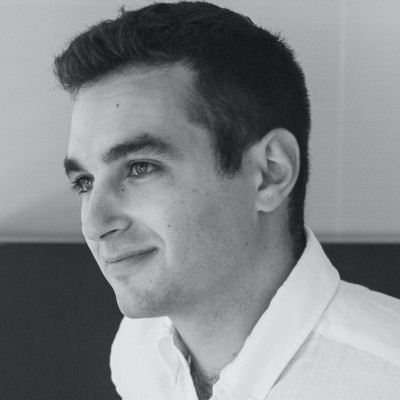
\includegraphics[width=3.2cm]{figures/author.png}
\end{flushright}

\vspace{-1em}

\noindent Joseph Gideon Meyer was born in Toronto, Ontario, Canada. He studied
Electrical Engineering at Tel Aviv University (TAU), receiving his BSc in 2022 and his
MSc in 2024. His master's research, supervised by Prof.\ Ady Arie, addressed
free-space quantum key distribution via spatial modes of light.

\vspace{0.6em}

\noindent Alongside his academic training, from 2021 to 2025 he worked as an
FPGA engineer at Elisra, where he contributed to chip design and algorithm
development and gained hands-on experience with the programmable hardware that
later became central to his doctoral research.

\vspace{0.6em}

\noindent From 2025 to 2026 he pursued a PhD within the QUARC doctoral network,
funded by the Marie Sk\l{}odowska-Curie Actions, as an industrial doctorate at
Eindhoven University of Technology (TU/e) under the supervision of
prof.dr.ir.\ I.~Tafur Monroy and embedded with NVIDIA's networking organization.
His research, carried out at the intersection of integrated photonics,
cryptography, and programmable datacenter hardware, forms the basis of this
dissertation on cross-layer network security in the post-quantum era.

\vspace{0.6em}

\noindent Since 2026 he has been a senior network researcher at NVIDIA, where he
continues to work on quantum-resilient and high-performance networking.


\chapter{Bibliography}
\label{bibliography}
\sloppy
\printbibliography[notkeyword={my_contribution}, heading=none]

\end{document}
